\documentclass[11pt, twoside]{article}

	\date{\LaTeX, Puteaux, 2020, 2021}
	\usepackage{fancyhdr}
	\usepackage{lastpage}
	\let\titleoriginal\title
	\renewcommand{\title}[1]{
		\titleoriginal{#1}
		\newcommand{\thetitle}{#1}}
	\fancypagestyle{plain}{
		\fancyhf{}
		\renewcommand{\headrulewidth}{0pt}
		\fancyfootoffset[RE]{-0.25\textwidth}
		\fancyfoot[R]{Page \thepage\ of \pageref{LastPage}}}
	\pagestyle{fancy}
	\fancyhf{}
	\renewcommand{\footrulewidth}{0.5pt}
	\fancyheadoffset[RE, LO]{-0.25\textwidth}
	\fancyfootoffset[RE, LO]{-0.25\textwidth}
	\fancyhead[LE,RO]{\thetitle}
	\fancyfoot[LE,RO]{Page \thepage\ of \pageref{LastPage}}
	\usepackage{wallpaper}
	\CenterWallPaper{}{../Figures/0. Wallpaper.jpg}

    \usepackage[breakable]{tcolorbox}
    \usepackage{parskip} % Stop auto-indenting (to mimic markdown behaviour)
    
    \usepackage{iftex}
    \ifPDFTeX
    	\usepackage[T1]{fontenc}
    	\usepackage{mathpazo}
    \else
    	\usepackage{fontspec}
    \fi

    % Basic figure setup, for now with no caption control since it's done
    % automatically by Pandoc (which extracts ![](path) syntax from Markdown).
    \usepackage{graphicx}
    % Maintain compatibility with old templates. Remove in nbconvert 6.0
    \let\Oldincludegraphics\includegraphics
    % Ensure that by default, figures have no caption (until we provide a
    % proper Figure object with a Caption API and a way to capture that
    % in the conversion process - todo).
    \usepackage{caption}
    \DeclareCaptionFormat{nocaption}{}
    \captionsetup{format=nocaption,aboveskip=0pt,belowskip=0pt}

    \usepackage[Export]{adjustbox} % Used to constrain images to a maximum size
    \adjustboxset{max size={0.9\linewidth}{0.9\paperheight}}
    \usepackage{float}
    \floatplacement{figure}{H} % forces figures to be placed at the correct location
    \usepackage{xcolor} % Allow colors to be defined
    \usepackage{enumerate} % Needed for markdown enumerations to work
    \usepackage{geometry} % Used to adjust the document margins
    \usepackage{amsmath} % Equations
    \usepackage{amssymb} % Equations
    \usepackage{textcomp} % defines textquotesingle
    % Hack from http://tex.stackexchange.com/a/47451/13684:
    \AtBeginDocument{%
        \def\PYZsq{\textquotesingle}% Upright quotes in Pygmentized code
    }
    \usepackage{upquote} % Upright quotes for verbatim code
    \usepackage{eurosym} % defines \euro
    \usepackage[mathletters]{ucs} % Extended unicode (utf-8) support
    \usepackage{fancyvrb} % verbatim replacement that allows latex
    \usepackage{grffile} % extends the file name processing of package graphics 
                         % to support a larger range
    \makeatletter % fix for grffile with XeLaTeX
    \def\Gread@@xetex#1{%
      \IfFileExists{"\Gin@base".bb}%
      {\Gread@eps{\Gin@base.bb}}%
      {\Gread@@xetex@aux#1}%
    }
    \makeatother

    % The hyperref package gives us a pdf with properly built
    % internal navigation ('pdf bookmarks' for the table of contents,
    % internal cross-reference links, web links for URLs, etc.)
    \usepackage{hyperref}
    % The default LaTeX title has an obnoxious amount of whitespace. By default,
    % titling removes some of it. It also provides customization options.
    \usepackage{titling}
    \usepackage{longtable} % longtable support required by pandoc >1.10
    \usepackage{booktabs}  % table support for pandoc > 1.12.2
    \usepackage[inline]{enumitem} % IRkernel/repr support (it uses the enumerate* environment)
    \usepackage[normalem]{ulem} % ulem is needed to support strikethroughs (\sout)
                                % normalem makes italics be italics, not underlines
    \usepackage{mathrsfs}
    

    
    % Colors for the hyperref package
    \definecolor{urlcolor}{rgb}{0,.145,.698}
    \definecolor{linkcolor}{rgb}{.71,0.21,0.01}
    \definecolor{citecolor}{rgb}{.12,.54,.11}

    % ANSI colors
    \definecolor{ansi-black}{HTML}{3E424D}
    \definecolor{ansi-black-intense}{HTML}{282C36}
    \definecolor{ansi-red}{HTML}{E75C58}
    \definecolor{ansi-red-intense}{HTML}{B22B31}
    \definecolor{ansi-green}{HTML}{00A250}
    \definecolor{ansi-green-intense}{HTML}{007427}
    \definecolor{ansi-yellow}{HTML}{DDB62B}
    \definecolor{ansi-yellow-intense}{HTML}{B27D12}
    \definecolor{ansi-blue}{HTML}{208FFB}
    \definecolor{ansi-blue-intense}{HTML}{0065CA}
    \definecolor{ansi-magenta}{HTML}{D160C4}
    \definecolor{ansi-magenta-intense}{HTML}{A03196}
    \definecolor{ansi-cyan}{HTML}{60C6C8}
    \definecolor{ansi-cyan-intense}{HTML}{258F8F}
    \definecolor{ansi-white}{HTML}{C5C1B4}
    \definecolor{ansi-white-intense}{HTML}{A1A6B2}
    \definecolor{ansi-default-inverse-fg}{HTML}{FFFFFF}
    \definecolor{ansi-default-inverse-bg}{HTML}{000000}

    % commands and environments needed by pandoc snippets
    % extracted from the output of `pandoc -s`
    \providecommand{\tightlist}{%
      \setlength{\itemsep}{0pt}\setlength{\parskip}{0pt}}
    \DefineVerbatimEnvironment{Highlighting}{Verbatim}{commandchars=\\\{\}}
    % Add ',fontsize=\small' for more characters per line
    \newenvironment{Shaded}{}{}
    \newcommand{\KeywordTok}[1]{\textcolor[rgb]{0.00,0.44,0.13}{\textbf{{#1}}}}
    \newcommand{\DataTypeTok}[1]{\textcolor[rgb]{0.56,0.13,0.00}{{#1}}}
    \newcommand{\DecValTok}[1]{\textcolor[rgb]{0.25,0.63,0.44}{{#1}}}
    \newcommand{\BaseNTok}[1]{\textcolor[rgb]{0.25,0.63,0.44}{{#1}}}
    \newcommand{\FloatTok}[1]{\textcolor[rgb]{0.25,0.63,0.44}{{#1}}}
    \newcommand{\CharTok}[1]{\textcolor[rgb]{0.25,0.44,0.63}{{#1}}}
    \newcommand{\StringTok}[1]{\textcolor[rgb]{0.25,0.44,0.63}{{#1}}}
    \newcommand{\CommentTok}[1]{\textcolor[rgb]{0.38,0.63,0.69}{\textit{{#1}}}}
    \newcommand{\OtherTok}[1]{\textcolor[rgb]{0.00,0.44,0.13}{{#1}}}
    \newcommand{\AlertTok}[1]{\textcolor[rgb]{1.00,0.00,0.00}{\textbf{{#1}}}}
    \newcommand{\FunctionTok}[1]{\textcolor[rgb]{0.02,0.16,0.49}{{#1}}}
    \newcommand{\RegionMarkerTok}[1]{{#1}}
    \newcommand{\ErrorTok}[1]{\textcolor[rgb]{1.00,0.00,0.00}{\textbf{{#1}}}}
    \newcommand{\NormalTok}[1]{{#1}}
    
    % Additional commands for more recent versions of Pandoc
    \newcommand{\ConstantTok}[1]{\textcolor[rgb]{0.53,0.00,0.00}{{#1}}}
    \newcommand{\SpecialCharTok}[1]{\textcolor[rgb]{0.25,0.44,0.63}{{#1}}}
    \newcommand{\VerbatimStringTok}[1]{\textcolor[rgb]{0.25,0.44,0.63}{{#1}}}
    \newcommand{\SpecialStringTok}[1]{\textcolor[rgb]{0.73,0.40,0.53}{{#1}}}
    \newcommand{\ImportTok}[1]{{#1}}
    \newcommand{\DocumentationTok}[1]{\textcolor[rgb]{0.73,0.13,0.13}{\textit{{#1}}}}
    \newcommand{\AnnotationTok}[1]{\textcolor[rgb]{0.38,0.63,0.69}{\textbf{\textit{{#1}}}}}
    \newcommand{\CommentVarTok}[1]{\textcolor[rgb]{0.38,0.63,0.69}{\textbf{\textit{{#1}}}}}
    \newcommand{\VariableTok}[1]{\textcolor[rgb]{0.10,0.09,0.49}{{#1}}}
    \newcommand{\ControlFlowTok}[1]{\textcolor[rgb]{0.00,0.44,0.13}{\textbf{{#1}}}}
    \newcommand{\OperatorTok}[1]{\textcolor[rgb]{0.40,0.40,0.40}{{#1}}}
    \newcommand{\BuiltInTok}[1]{{#1}}
    \newcommand{\ExtensionTok}[1]{{#1}}
    \newcommand{\PreprocessorTok}[1]{\textcolor[rgb]{0.74,0.48,0.00}{{#1}}}
    \newcommand{\AttributeTok}[1]{\textcolor[rgb]{0.49,0.56,0.16}{{#1}}}
    \newcommand{\InformationTok}[1]{\textcolor[rgb]{0.38,0.63,0.69}{\textbf{\textit{{#1}}}}}
    \newcommand{\WarningTok}[1]{\textcolor[rgb]{0.38,0.63,0.69}{\textbf{\textit{{#1}}}}}
    
    
    % Define a nice break command that doesn't care if a line doesn't already
    % exist.
    \def\br{\hspace*{\fill} \\* }
    % Math Jax compatibility definitions
    \def\gt{>}
    \def\lt{<}
    \let\Oldtex\TeX
    \let\Oldlatex\LaTeX
    \renewcommand{\TeX}{\textrm{\Oldtex}}
    \renewcommand{\LaTeX}{\textrm{\Oldlatex}}
    % Document parameters
    % Document title
    \title{Fine-Tuning Keras Models}
    
    
    
    
    
% Pygments definitions
\makeatletter
\def\PY@reset{\let\PY@it=\relax \let\PY@bf=\relax%
    \let\PY@ul=\relax \let\PY@tc=\relax%
    \let\PY@bc=\relax \let\PY@ff=\relax}
\def\PY@tok#1{\csname PY@tok@#1\endcsname}
\def\PY@toks#1+{\ifx\relax#1\empty\else%
    \PY@tok{#1}\expandafter\PY@toks\fi}
\def\PY@do#1{\PY@bc{\PY@tc{\PY@ul{%
    \PY@it{\PY@bf{\PY@ff{#1}}}}}}}
\def\PY#1#2{\PY@reset\PY@toks#1+\relax+\PY@do{#2}}

\expandafter\def\csname PY@tok@w\endcsname{\def\PY@tc##1{\textcolor[rgb]{0.73,0.73,0.73}{##1}}}
\expandafter\def\csname PY@tok@c\endcsname{\let\PY@it=\textit\def\PY@tc##1{\textcolor[rgb]{0.25,0.50,0.50}{##1}}}
\expandafter\def\csname PY@tok@cp\endcsname{\def\PY@tc##1{\textcolor[rgb]{0.74,0.48,0.00}{##1}}}
\expandafter\def\csname PY@tok@k\endcsname{\let\PY@bf=\textbf\def\PY@tc##1{\textcolor[rgb]{0.00,0.50,0.00}{##1}}}
\expandafter\def\csname PY@tok@kp\endcsname{\def\PY@tc##1{\textcolor[rgb]{0.00,0.50,0.00}{##1}}}
\expandafter\def\csname PY@tok@kt\endcsname{\def\PY@tc##1{\textcolor[rgb]{0.69,0.00,0.25}{##1}}}
\expandafter\def\csname PY@tok@o\endcsname{\def\PY@tc##1{\textcolor[rgb]{0.40,0.40,0.40}{##1}}}
\expandafter\def\csname PY@tok@ow\endcsname{\let\PY@bf=\textbf\def\PY@tc##1{\textcolor[rgb]{0.67,0.13,1.00}{##1}}}
\expandafter\def\csname PY@tok@nb\endcsname{\def\PY@tc##1{\textcolor[rgb]{0.00,0.50,0.00}{##1}}}
\expandafter\def\csname PY@tok@nf\endcsname{\def\PY@tc##1{\textcolor[rgb]{0.00,0.00,1.00}{##1}}}
\expandafter\def\csname PY@tok@nc\endcsname{\let\PY@bf=\textbf\def\PY@tc##1{\textcolor[rgb]{0.00,0.00,1.00}{##1}}}
\expandafter\def\csname PY@tok@nn\endcsname{\let\PY@bf=\textbf\def\PY@tc##1{\textcolor[rgb]{0.00,0.00,1.00}{##1}}}
\expandafter\def\csname PY@tok@ne\endcsname{\let\PY@bf=\textbf\def\PY@tc##1{\textcolor[rgb]{0.82,0.25,0.23}{##1}}}
\expandafter\def\csname PY@tok@nv\endcsname{\def\PY@tc##1{\textcolor[rgb]{0.10,0.09,0.49}{##1}}}
\expandafter\def\csname PY@tok@no\endcsname{\def\PY@tc##1{\textcolor[rgb]{0.53,0.00,0.00}{##1}}}
\expandafter\def\csname PY@tok@nl\endcsname{\def\PY@tc##1{\textcolor[rgb]{0.63,0.63,0.00}{##1}}}
\expandafter\def\csname PY@tok@ni\endcsname{\let\PY@bf=\textbf\def\PY@tc##1{\textcolor[rgb]{0.60,0.60,0.60}{##1}}}
\expandafter\def\csname PY@tok@na\endcsname{\def\PY@tc##1{\textcolor[rgb]{0.49,0.56,0.16}{##1}}}
\expandafter\def\csname PY@tok@nt\endcsname{\let\PY@bf=\textbf\def\PY@tc##1{\textcolor[rgb]{0.00,0.50,0.00}{##1}}}
\expandafter\def\csname PY@tok@nd\endcsname{\def\PY@tc##1{\textcolor[rgb]{0.67,0.13,1.00}{##1}}}
\expandafter\def\csname PY@tok@s\endcsname{\def\PY@tc##1{\textcolor[rgb]{0.73,0.13,0.13}{##1}}}
\expandafter\def\csname PY@tok@sd\endcsname{\let\PY@it=\textit\def\PY@tc##1{\textcolor[rgb]{0.73,0.13,0.13}{##1}}}
\expandafter\def\csname PY@tok@si\endcsname{\let\PY@bf=\textbf\def\PY@tc##1{\textcolor[rgb]{0.73,0.40,0.53}{##1}}}
\expandafter\def\csname PY@tok@se\endcsname{\let\PY@bf=\textbf\def\PY@tc##1{\textcolor[rgb]{0.73,0.40,0.13}{##1}}}
\expandafter\def\csname PY@tok@sr\endcsname{\def\PY@tc##1{\textcolor[rgb]{0.73,0.40,0.53}{##1}}}
\expandafter\def\csname PY@tok@ss\endcsname{\def\PY@tc##1{\textcolor[rgb]{0.10,0.09,0.49}{##1}}}
\expandafter\def\csname PY@tok@sx\endcsname{\def\PY@tc##1{\textcolor[rgb]{0.00,0.50,0.00}{##1}}}
\expandafter\def\csname PY@tok@m\endcsname{\def\PY@tc##1{\textcolor[rgb]{0.40,0.40,0.40}{##1}}}
\expandafter\def\csname PY@tok@gh\endcsname{\let\PY@bf=\textbf\def\PY@tc##1{\textcolor[rgb]{0.00,0.00,0.50}{##1}}}
\expandafter\def\csname PY@tok@gu\endcsname{\let\PY@bf=\textbf\def\PY@tc##1{\textcolor[rgb]{0.50,0.00,0.50}{##1}}}
\expandafter\def\csname PY@tok@gd\endcsname{\def\PY@tc##1{\textcolor[rgb]{0.63,0.00,0.00}{##1}}}
\expandafter\def\csname PY@tok@gi\endcsname{\def\PY@tc##1{\textcolor[rgb]{0.00,0.63,0.00}{##1}}}
\expandafter\def\csname PY@tok@gr\endcsname{\def\PY@tc##1{\textcolor[rgb]{1.00,0.00,0.00}{##1}}}
\expandafter\def\csname PY@tok@ge\endcsname{\let\PY@it=\textit}
\expandafter\def\csname PY@tok@gs\endcsname{\let\PY@bf=\textbf}
\expandafter\def\csname PY@tok@gp\endcsname{\let\PY@bf=\textbf\def\PY@tc##1{\textcolor[rgb]{0.00,0.00,0.50}{##1}}}
\expandafter\def\csname PY@tok@go\endcsname{\def\PY@tc##1{\textcolor[rgb]{0.53,0.53,0.53}{##1}}}
\expandafter\def\csname PY@tok@gt\endcsname{\def\PY@tc##1{\textcolor[rgb]{0.00,0.27,0.87}{##1}}}
\expandafter\def\csname PY@tok@err\endcsname{\def\PY@bc##1{\setlength{\fboxsep}{0pt}\fcolorbox[rgb]{1.00,0.00,0.00}{1,1,1}{\strut ##1}}}
\expandafter\def\csname PY@tok@kc\endcsname{\let\PY@bf=\textbf\def\PY@tc##1{\textcolor[rgb]{0.00,0.50,0.00}{##1}}}
\expandafter\def\csname PY@tok@kd\endcsname{\let\PY@bf=\textbf\def\PY@tc##1{\textcolor[rgb]{0.00,0.50,0.00}{##1}}}
\expandafter\def\csname PY@tok@kn\endcsname{\let\PY@bf=\textbf\def\PY@tc##1{\textcolor[rgb]{0.00,0.50,0.00}{##1}}}
\expandafter\def\csname PY@tok@kr\endcsname{\let\PY@bf=\textbf\def\PY@tc##1{\textcolor[rgb]{0.00,0.50,0.00}{##1}}}
\expandafter\def\csname PY@tok@bp\endcsname{\def\PY@tc##1{\textcolor[rgb]{0.00,0.50,0.00}{##1}}}
\expandafter\def\csname PY@tok@fm\endcsname{\def\PY@tc##1{\textcolor[rgb]{0.00,0.00,1.00}{##1}}}
\expandafter\def\csname PY@tok@vc\endcsname{\def\PY@tc##1{\textcolor[rgb]{0.10,0.09,0.49}{##1}}}
\expandafter\def\csname PY@tok@vg\endcsname{\def\PY@tc##1{\textcolor[rgb]{0.10,0.09,0.49}{##1}}}
\expandafter\def\csname PY@tok@vi\endcsname{\def\PY@tc##1{\textcolor[rgb]{0.10,0.09,0.49}{##1}}}
\expandafter\def\csname PY@tok@vm\endcsname{\def\PY@tc##1{\textcolor[rgb]{0.10,0.09,0.49}{##1}}}
\expandafter\def\csname PY@tok@sa\endcsname{\def\PY@tc##1{\textcolor[rgb]{0.73,0.13,0.13}{##1}}}
\expandafter\def\csname PY@tok@sb\endcsname{\def\PY@tc##1{\textcolor[rgb]{0.73,0.13,0.13}{##1}}}
\expandafter\def\csname PY@tok@sc\endcsname{\def\PY@tc##1{\textcolor[rgb]{0.73,0.13,0.13}{##1}}}
\expandafter\def\csname PY@tok@dl\endcsname{\def\PY@tc##1{\textcolor[rgb]{0.73,0.13,0.13}{##1}}}
\expandafter\def\csname PY@tok@s2\endcsname{\def\PY@tc##1{\textcolor[rgb]{0.73,0.13,0.13}{##1}}}
\expandafter\def\csname PY@tok@sh\endcsname{\def\PY@tc##1{\textcolor[rgb]{0.73,0.13,0.13}{##1}}}
\expandafter\def\csname PY@tok@s1\endcsname{\def\PY@tc##1{\textcolor[rgb]{0.73,0.13,0.13}{##1}}}
\expandafter\def\csname PY@tok@mb\endcsname{\def\PY@tc##1{\textcolor[rgb]{0.40,0.40,0.40}{##1}}}
\expandafter\def\csname PY@tok@mf\endcsname{\def\PY@tc##1{\textcolor[rgb]{0.40,0.40,0.40}{##1}}}
\expandafter\def\csname PY@tok@mh\endcsname{\def\PY@tc##1{\textcolor[rgb]{0.40,0.40,0.40}{##1}}}
\expandafter\def\csname PY@tok@mi\endcsname{\def\PY@tc##1{\textcolor[rgb]{0.40,0.40,0.40}{##1}}}
\expandafter\def\csname PY@tok@il\endcsname{\def\PY@tc##1{\textcolor[rgb]{0.40,0.40,0.40}{##1}}}
\expandafter\def\csname PY@tok@mo\endcsname{\def\PY@tc##1{\textcolor[rgb]{0.40,0.40,0.40}{##1}}}
\expandafter\def\csname PY@tok@ch\endcsname{\let\PY@it=\textit\def\PY@tc##1{\textcolor[rgb]{0.25,0.50,0.50}{##1}}}
\expandafter\def\csname PY@tok@cm\endcsname{\let\PY@it=\textit\def\PY@tc##1{\textcolor[rgb]{0.25,0.50,0.50}{##1}}}
\expandafter\def\csname PY@tok@cpf\endcsname{\let\PY@it=\textit\def\PY@tc##1{\textcolor[rgb]{0.25,0.50,0.50}{##1}}}
\expandafter\def\csname PY@tok@c1\endcsname{\let\PY@it=\textit\def\PY@tc##1{\textcolor[rgb]{0.25,0.50,0.50}{##1}}}
\expandafter\def\csname PY@tok@cs\endcsname{\let\PY@it=\textit\def\PY@tc##1{\textcolor[rgb]{0.25,0.50,0.50}{##1}}}

\def\PYZbs{\char`\\}
\def\PYZus{\char`\_}
\def\PYZob{\char`\{}
\def\PYZcb{\char`\}}
\def\PYZca{\char`\^}
\def\PYZam{\char`\&}
\def\PYZlt{\char`\<}
\def\PYZgt{\char`\>}
\def\PYZsh{\char`\#}
\def\PYZpc{\char`\%}
\def\PYZdl{\char`\$}
\def\PYZhy{\char`\-}
\def\PYZsq{\char`\'}
\def\PYZdq{\char`\"}
\def\PYZti{\char`\~}
% for compatibility with earlier versions
\def\PYZat{@}
\def\PYZlb{[}
\def\PYZrb{]}
\makeatother


    % For linebreaks inside Verbatim environment from package fancyvrb. 
    \makeatletter
        \newbox\Wrappedcontinuationbox 
        \newbox\Wrappedvisiblespacebox 
        \newcommand*\Wrappedvisiblespace {\textcolor{red}{\textvisiblespace}} 
        \newcommand*\Wrappedcontinuationsymbol {\textcolor{red}{\llap{\tiny$\m@th\hookrightarrow$}}} 
        \newcommand*\Wrappedcontinuationindent {3ex } 
        \newcommand*\Wrappedafterbreak {\kern\Wrappedcontinuationindent\copy\Wrappedcontinuationbox} 
        % Take advantage of the already applied Pygments mark-up to insert 
        % potential linebreaks for TeX processing. 
        %        {, <, #, %, $, ' and ": go to next line. 
        %        _, }, ^, &, >, - and ~: stay at end of broken line. 
        % Use of \textquotesingle for straight quote. 
        \newcommand*\Wrappedbreaksatspecials {% 
            \def\PYGZus{\discretionary{\char`\_}{\Wrappedafterbreak}{\char`\_}}% 
            \def\PYGZob{\discretionary{}{\Wrappedafterbreak\char`\{}{\char`\{}}% 
            \def\PYGZcb{\discretionary{\char`\}}{\Wrappedafterbreak}{\char`\}}}% 
            \def\PYGZca{\discretionary{\char`\^}{\Wrappedafterbreak}{\char`\^}}% 
            \def\PYGZam{\discretionary{\char`\&}{\Wrappedafterbreak}{\char`\&}}% 
            \def\PYGZlt{\discretionary{}{\Wrappedafterbreak\char`\<}{\char`\<}}% 
            \def\PYGZgt{\discretionary{\char`\>}{\Wrappedafterbreak}{\char`\>}}% 
            \def\PYGZsh{\discretionary{}{\Wrappedafterbreak\char`\#}{\char`\#}}% 
            \def\PYGZpc{\discretionary{}{\Wrappedafterbreak\char`\%}{\char`\%}}% 
            \def\PYGZdl{\discretionary{}{\Wrappedafterbreak\char`\$}{\char`\$}}% 
            \def\PYGZhy{\discretionary{\char`\-}{\Wrappedafterbreak}{\char`\-}}% 
            \def\PYGZsq{\discretionary{}{\Wrappedafterbreak\textquotesingle}{\textquotesingle}}% 
            \def\PYGZdq{\discretionary{}{\Wrappedafterbreak\char`\"}{\char`\"}}% 
            \def\PYGZti{\discretionary{\char`\~}{\Wrappedafterbreak}{\char`\~}}% 
        } 
        % Some characters . , ; ? ! / are not pygmentized. 
        % This macro makes them "active" and they will insert potential linebreaks 
        \newcommand*\Wrappedbreaksatpunct {% 
            \lccode`\~`\.\lowercase{\def~}{\discretionary{\hbox{\char`\.}}{\Wrappedafterbreak}{\hbox{\char`\.}}}% 
            \lccode`\~`\,\lowercase{\def~}{\discretionary{\hbox{\char`\,}}{\Wrappedafterbreak}{\hbox{\char`\,}}}% 
            \lccode`\~`\;\lowercase{\def~}{\discretionary{\hbox{\char`\;}}{\Wrappedafterbreak}{\hbox{\char`\;}}}% 
            \lccode`\~`\:\lowercase{\def~}{\discretionary{\hbox{\char`\:}}{\Wrappedafterbreak}{\hbox{\char`\:}}}% 
            \lccode`\~`\?\lowercase{\def~}{\discretionary{\hbox{\char`\?}}{\Wrappedafterbreak}{\hbox{\char`\?}}}% 
            \lccode`\~`\!\lowercase{\def~}{\discretionary{\hbox{\char`\!}}{\Wrappedafterbreak}{\hbox{\char`\!}}}% 
            \lccode`\~`\/\lowercase{\def~}{\discretionary{\hbox{\char`\/}}{\Wrappedafterbreak}{\hbox{\char`\/}}}% 
            \catcode`\.\active
            \catcode`\,\active 
            \catcode`\;\active
            \catcode`\:\active
            \catcode`\?\active
            \catcode`\!\active
            \catcode`\/\active 
            \lccode`\~`\~ 	
        }
    \makeatother

    \let\OriginalVerbatim=\Verbatim
    \makeatletter
    \renewcommand{\Verbatim}[1][1]{%
        %\parskip\z@skip
        \sbox\Wrappedcontinuationbox {\Wrappedcontinuationsymbol}%
        \sbox\Wrappedvisiblespacebox {\FV@SetupFont\Wrappedvisiblespace}%
        \def\FancyVerbFormatLine ##1{\hsize\linewidth
            \vtop{\raggedright\hyphenpenalty\z@\exhyphenpenalty\z@
                \doublehyphendemerits\z@\finalhyphendemerits\z@
                \strut ##1\strut}%
        }%
        % If the linebreak is at a space, the latter will be displayed as visible
        % space at end of first line, and a continuation symbol starts next line.
        % Stretch/shrink are however usually zero for typewriter font.
        \def\FV@Space {%
            \nobreak\hskip\z@ plus\fontdimen3\font minus\fontdimen4\font
            \discretionary{\copy\Wrappedvisiblespacebox}{\Wrappedafterbreak}
            {\kern\fontdimen2\font}%
        }%
        
        % Allow breaks at special characters using \PYG... macros.
        \Wrappedbreaksatspecials
        % Breaks at punctuation characters . , ; ? ! and / need catcode=\active 	
        \OriginalVerbatim[#1,codes*=\Wrappedbreaksatpunct]%
    }
    \makeatother

    % Exact colors from NB
    \definecolor{incolor}{HTML}{303F9F}
    \definecolor{outcolor}{HTML}{D84315}
    \definecolor{cellborder}{HTML}{CFCFCF}
    \definecolor{cellbackground}{HTML}{F7F7F7}
    
    % prompt
    \makeatletter
    \newcommand{\boxspacing}{\kern\kvtcb@left@rule\kern\kvtcb@boxsep}
    \makeatother
    \newcommand{\prompt}[4]{
        \ttfamily\llap{{\color{#2}[#3]:\hspace{3pt}#4}}\vspace{-\baselineskip}
    }
    

    
    % Prevent overflowing lines due to hard-to-break entities
    \sloppy 
    % Setup hyperref package
    \hypersetup{
      breaklinks=true,  % so long urls are correctly broken across lines
      colorlinks=true,
      urlcolor=urlcolor,
      linkcolor=linkcolor,
      citecolor=citecolor,
      }
    % Slightly bigger margins than the latex defaults
    
    \geometry{verbose,tmargin=1in,bmargin=1in,lmargin=1in,rmargin=1in}
    
    

\begin{document}
    
    \maketitle
    
    

    
    Table of Contents{}

{{1~~}Understanding model optimization}

{{1.1~~}{[}note-1{]} Why optimization is hard}

{{1.2~~}{[}code-1{]} Stochastic gradient descent}

{{1.3~~}{[}note-2{]} The dying neuron problem}

{{1.4~~}{[}note-3{]} Vanishing gradients}

{{1.5~~}{[}quiz-1{]} Diagnosing optimization problems}

{{1.6~~}{[}task-1{]} Changing optimization parameters}

{{2~~}Model validation}

{{2.1~~}{[}note-1{]} Validation in deep learning}

{{2.2~~}{[}code-1{]} Model validation}

{{2.3~~}{[}code-2{]} Early stopping}

{{2.4~~}{[}note-2{]} Experimentation}

{{2.5~~}{[}task-1{]} Evaluating model accuracy on a validation dataset}

{{2.6~~}{[}task-2{]} Early stopping: optimizing the optimization}

{{2.7~~}{[}task-3{]} Experimenting with wider networks}

{{2.8~~}{[}task-4{]} Adding layers to a network}

{{3~~}Thinking about model capacity}

{{3.1~~}{[}note-1{]} Overfitting}

{{3.2~~}{[}note-2{]} Workflow for optimizing model capacity}

{{3.3~~}{[}note-3{]} Sequential experiments}

{{3.4~~}{[}quiz-1{]} Experimenting with model structures}

{{4~~}Stepping up to images}

{{4.1~~}{[}note-1{]} Recognizing handwritten digits}

{{4.2~~}{[}task-1{]} Building an own digit recognition model}

{{5~~}Final thoughts}

{{5.1~~}{[}note-1{]} Next steps}

{{6~~}Requirements}

    \hypertarget{understanding-model-optimization}{%
\section{Understanding model
optimization}\label{understanding-model-optimization}}

    \hypertarget{note-1-why-optimization-is-hard}{%
\subsection{\texorpdfstring{\texttt{{[}note-1{]}} Why optimization is
hard}{{[}note-1{]} Why optimization is hard}}\label{note-1-why-optimization-is-hard}}

\begin{itemize}
\item
  Simultaneously optimizing 1000s of parameters with complex
  relationships.
\item
  Updates may not improve the model meaningfully.
\item
  Updates could be too small (if the learning rate is low) or too large
  (if the learning rate is high).
\end{itemize}

    \hypertarget{code-1-stochastic-gradient-descent}{%
\subsection{\texorpdfstring{\texttt{{[}code-1{]}} Stochastic gradient
descent}{{[}code-1{]} Stochastic gradient descent}}\label{code-1-stochastic-gradient-descent}}

    \begin{tcolorbox}[breakable, size=fbox, boxrule=1pt, pad at break*=1mm,colback=cellbackground, colframe=cellborder]
\prompt{In}{incolor}{1}{\boxspacing}
\begin{Verbatim}[commandchars=\\\{\}]
\PY{k+kn}{import} \PY{n+nn}{pandas} \PY{k}{as} \PY{n+nn}{pd}
\PY{k+kn}{from} \PY{n+nn}{tensorflow}\PY{n+nn}{.}\PY{n+nn}{keras}\PY{n+nn}{.}\PY{n+nn}{layers} \PY{k+kn}{import} \PY{n}{Dense}
\PY{k+kn}{from} \PY{n+nn}{tensorflow}\PY{n+nn}{.}\PY{n+nn}{keras}\PY{n+nn}{.}\PY{n+nn}{models} \PY{k+kn}{import} \PY{n}{Sequential}
\PY{k+kn}{from} \PY{n+nn}{tensorflow}\PY{n+nn}{.}\PY{n+nn}{keras}\PY{n+nn}{.}\PY{n+nn}{utils} \PY{k+kn}{import} \PY{n}{to\PYZus{}categorical}
\PY{k+kn}{from} \PY{n+nn}{tensorflow}\PY{n+nn}{.}\PY{n+nn}{keras}\PY{n+nn}{.}\PY{n+nn}{optimizers} \PY{k+kn}{import} \PY{n}{SGD}


\PY{k}{def} \PY{n+nf}{data\PYZus{}preparation}\PY{p}{(}\PY{n}{data}\PY{p}{)}\PY{p}{:}
    \PY{n}{df} \PY{o}{=} \PY{n}{data}\PY{o}{.}\PY{n}{reindex}\PY{p}{(}\PY{n}{columns}\PY{o}{=}\PY{p}{[}
        \PY{l+s+s1}{\PYZsq{}}\PY{l+s+s1}{SHOT\PYZus{}CLOCK}\PY{l+s+s1}{\PYZsq{}}\PY{p}{,} \PY{l+s+s1}{\PYZsq{}}\PY{l+s+s1}{DRIBBLES}\PY{l+s+s1}{\PYZsq{}}\PY{p}{,} \PY{l+s+s1}{\PYZsq{}}\PY{l+s+s1}{TOUCH\PYZus{}TIME}\PY{l+s+s1}{\PYZsq{}}\PY{p}{,} \PY{l+s+s1}{\PYZsq{}}\PY{l+s+s1}{SHOT\PYZus{}DIST}\PY{l+s+s1}{\PYZsq{}}\PY{p}{,} \PY{l+s+s1}{\PYZsq{}}\PY{l+s+s1}{CLOSE\PYZus{}DEF\PYZus{}DIST}\PY{l+s+s1}{\PYZsq{}}\PY{p}{,}
        \PY{l+s+s1}{\PYZsq{}}\PY{l+s+s1}{SHOT\PYZus{}RESULT}\PY{l+s+s1}{\PYZsq{}}
    \PY{p}{]}\PY{p}{)}
    \PY{n}{df}\PY{p}{[}\PY{l+s+s1}{\PYZsq{}}\PY{l+s+s1}{SHOT\PYZus{}CLOCK}\PY{l+s+s1}{\PYZsq{}}\PY{p}{]} \PY{o}{=} \PY{n}{df}\PY{p}{[}\PY{l+s+s1}{\PYZsq{}}\PY{l+s+s1}{SHOT\PYZus{}CLOCK}\PY{l+s+s1}{\PYZsq{}}\PY{p}{]}\PY{o}{.}\PY{n}{fillna}\PY{p}{(}\PY{l+m+mi}{0}\PY{p}{)}
    \PY{n}{df}\PY{p}{[}\PY{l+s+s1}{\PYZsq{}}\PY{l+s+s1}{SHOT\PYZus{}RESULT}\PY{l+s+s1}{\PYZsq{}}\PY{p}{]}\PY{o}{.}\PY{n}{replace}\PY{p}{(}\PY{l+s+s1}{\PYZsq{}}\PY{l+s+s1}{missed}\PY{l+s+s1}{\PYZsq{}}\PY{p}{,} \PY{l+m+mi}{0}\PY{p}{,} \PY{n}{inplace}\PY{o}{=}\PY{k+kc}{True}\PY{p}{)}
    \PY{n}{df}\PY{p}{[}\PY{l+s+s1}{\PYZsq{}}\PY{l+s+s1}{SHOT\PYZus{}RESULT}\PY{l+s+s1}{\PYZsq{}}\PY{p}{]}\PY{o}{.}\PY{n}{replace}\PY{p}{(}\PY{l+s+s1}{\PYZsq{}}\PY{l+s+s1}{made}\PY{l+s+s1}{\PYZsq{}}\PY{p}{,} \PY{l+m+mi}{1}\PY{p}{,} \PY{n}{inplace}\PY{o}{=}\PY{k+kc}{True}\PY{p}{)}
    \PY{n}{df}\PY{o}{.}\PY{n}{columns} \PY{o}{=} \PY{n}{df}\PY{o}{.}\PY{n}{columns}\PY{o}{.}\PY{n}{str}\PY{o}{.}\PY{n}{lower}\PY{p}{(}\PY{p}{)}
    \PY{k}{return} \PY{n}{df}


\PY{n}{data} \PY{o}{=} \PY{n}{pd}\PY{o}{.}\PY{n}{read\PYZus{}csv}\PY{p}{(}\PY{l+s+s1}{\PYZsq{}}\PY{l+s+s1}{../Datasets/1. Basketball shot log.csv}\PY{l+s+s1}{\PYZsq{}}\PY{p}{)}
\PY{n}{df} \PY{o}{=} \PY{n}{data\PYZus{}preparation}\PY{p}{(}\PY{n}{data}\PY{p}{)}

\PY{n}{predictors} \PY{o}{=} \PY{n}{df}\PY{o}{.}\PY{n}{drop}\PY{p}{(}\PY{p}{[}\PY{l+s+s1}{\PYZsq{}}\PY{l+s+s1}{shot\PYZus{}result}\PY{l+s+s1}{\PYZsq{}}\PY{p}{]}\PY{p}{,} \PY{n}{axis}\PY{o}{=}\PY{l+m+mi}{1}\PY{p}{)}\PY{o}{.}\PY{n}{to\PYZus{}numpy}\PY{p}{(}\PY{p}{)}
\PY{n}{n\PYZus{}cols} \PY{o}{=} \PY{n}{predictors}\PY{o}{.}\PY{n}{shape}\PY{p}{[}\PY{l+m+mi}{1}\PY{p}{]}
\PY{n}{target} \PY{o}{=} \PY{n}{to\PYZus{}categorical}\PY{p}{(}\PY{n}{df}\PY{o}{.}\PY{n}{shot\PYZus{}result}\PY{p}{)}
\PY{n}{input\PYZus{}shape} \PY{o}{=} \PY{p}{(}\PY{n}{n\PYZus{}cols}\PY{p}{,} \PY{p}{)}


\PY{k}{def} \PY{n+nf}{get\PYZus{}new\PYZus{}model}\PY{p}{(}\PY{n}{input\PYZus{}shape}\PY{o}{=}\PY{n}{input\PYZus{}shape}\PY{p}{)}\PY{p}{:}
    \PY{n}{model} \PY{o}{=} \PY{n}{Sequential}\PY{p}{(}\PY{p}{)}
    \PY{n}{model}\PY{o}{.}\PY{n}{add}\PY{p}{(}\PY{n}{Dense}\PY{p}{(}\PY{l+m+mi}{100}\PY{p}{,} \PY{n}{activation}\PY{o}{=}\PY{l+s+s1}{\PYZsq{}}\PY{l+s+s1}{relu}\PY{l+s+s1}{\PYZsq{}}\PY{p}{,} \PY{n}{input\PYZus{}shape}\PY{o}{=}\PY{n}{input\PYZus{}shape}\PY{p}{)}\PY{p}{)}
    \PY{n}{model}\PY{o}{.}\PY{n}{add}\PY{p}{(}\PY{n}{Dense}\PY{p}{(}\PY{l+m+mi}{100}\PY{p}{,} \PY{n}{activation}\PY{o}{=}\PY{l+s+s1}{\PYZsq{}}\PY{l+s+s1}{relu}\PY{l+s+s1}{\PYZsq{}}\PY{p}{)}\PY{p}{)}
    \PY{n}{model}\PY{o}{.}\PY{n}{add}\PY{p}{(}\PY{n}{Dense}\PY{p}{(}\PY{l+m+mi}{2}\PY{p}{,} \PY{n}{activation}\PY{o}{=}\PY{l+s+s1}{\PYZsq{}}\PY{l+s+s1}{softmax}\PY{l+s+s1}{\PYZsq{}}\PY{p}{)}\PY{p}{)}
    \PY{k}{return} \PY{p}{(}\PY{n}{model}\PY{p}{)}


\PY{n}{lr\PYZus{}to\PYZus{}test} \PY{o}{=} \PY{p}{[}\PY{o}{.}\PY{l+m+mi}{000001}\PY{p}{,} \PY{l+m+mf}{0.01}\PY{p}{,} \PY{l+m+mi}{1}\PY{p}{]}

\PY{c+c1}{\PYZsh{} loop over learning rates}
\PY{k}{for} \PY{n}{lr} \PY{o+ow}{in} \PY{n}{lr\PYZus{}to\PYZus{}test}\PY{p}{:}
    \PY{n}{model} \PY{o}{=} \PY{n}{get\PYZus{}new\PYZus{}model}\PY{p}{(}\PY{p}{)}
    \PY{n}{my\PYZus{}optimizer} \PY{o}{=} \PY{n}{SGD}\PY{p}{(}\PY{n}{lr}\PY{o}{=}\PY{n}{lr}\PY{p}{)}
    \PY{n}{model}\PY{o}{.}\PY{n}{compile}\PY{p}{(}\PY{n}{optimizer}\PY{o}{=}\PY{n}{my\PYZus{}optimizer}\PY{p}{,} \PY{n}{loss}\PY{o}{=}\PY{l+s+s1}{\PYZsq{}}\PY{l+s+s1}{categorical\PYZus{}crossentropy}\PY{l+s+s1}{\PYZsq{}}\PY{p}{)}
    \PY{n}{model}\PY{o}{.}\PY{n}{fit}\PY{p}{(}\PY{n}{predictors}\PY{p}{,} \PY{n}{target}\PY{p}{)}
\end{Verbatim}
\end{tcolorbox}

    \begin{Verbatim}[commandchars=\\\{\}]
4003/4003 [==============================] - 4s 958us/step - loss: 1.2821
4003/4003 [==============================] - 4s 937us/step - loss: 0.6770
4003/4003 [==============================] - 4s 954us/step - loss: nan
    \end{Verbatim}

    \hypertarget{note-2-the-dying-neuron-problem}{%
\subsection{\texorpdfstring{\texttt{{[}note-2{]}} The dying neuron
problem}{{[}note-2{]} The dying neuron problem}}\label{note-2-the-dying-neuron-problem}}

\begin{figure}
\centering

\includegraphics{../Figures/1. The dying neuron problem.jpg}
\caption{The dying neuron problem}
\end{figure}

    \hypertarget{note-3-vanishing-gradients}{%
\subsection{\texorpdfstring{\texttt{{[}note-3{]}} Vanishing
gradients}{{[}note-3{]} Vanishing gradients}}\label{note-3-vanishing-gradients}}

\begin{itemize}
\item
  It occurs when many layers have very small slopes (\emph{e.g., due to
  being on at part of tanh curve}).
\item
  In deep networks, updates to backpropagation were close to 0.
\end{itemize}

\begin{figure}
\centering
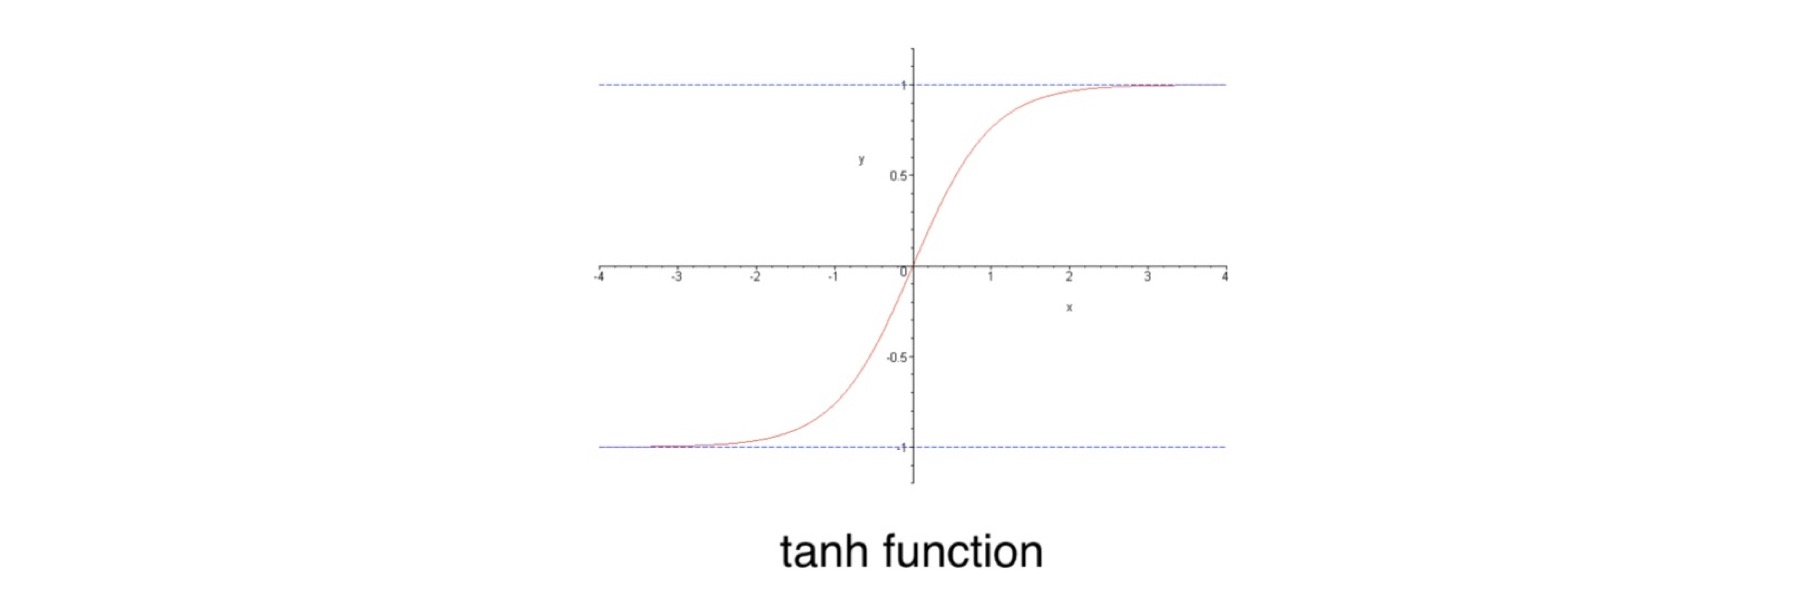
\includegraphics{../Figures/2. Vanishing gradient.jpg}
\caption{Vanishing gradients}
\end{figure}

    \hypertarget{quiz-1-diagnosing-optimization-problems}{%
\subsection{\texorpdfstring{\texttt{{[}quiz-1{]}} Diagnosing
optimization
problems}{{[}quiz-1{]} Diagnosing optimization problems}}\label{quiz-1-diagnosing-optimization-problems}}

\begin{itemize}
\item
  Which of the following could prevent a model from showing an improved
  loss in its first few epochs?

  \(\Box\) Learning rate too low.

  \(\Box\) Learning rate too high.

  \(\Box\) Poor choice of the activation function.

  \(\boxtimes\) All of the above.
\end{itemize}

    \hypertarget{task-1-changing-optimization-parameters}{%
\subsection{\texorpdfstring{\texttt{{[}task-1{]}} Changing optimization
parameters}{{[}task-1{]} Changing optimization parameters}}\label{task-1-changing-optimization-parameters}}

\(\blacktriangleright\) \textbf{Package pre-loading}

    \begin{tcolorbox}[breakable, size=fbox, boxrule=1pt, pad at break*=1mm,colback=cellbackground, colframe=cellborder]
\prompt{In}{incolor}{2}{\boxspacing}
\begin{Verbatim}[commandchars=\\\{\}]
\PY{k+kn}{import} \PY{n+nn}{pandas} \PY{k}{as} \PY{n+nn}{pd}
\PY{k+kn}{from} \PY{n+nn}{tensorflow}\PY{n+nn}{.}\PY{n+nn}{keras}\PY{n+nn}{.}\PY{n+nn}{layers} \PY{k+kn}{import} \PY{n}{Dense}
\PY{k+kn}{from} \PY{n+nn}{tensorflow}\PY{n+nn}{.}\PY{n+nn}{keras}\PY{n+nn}{.}\PY{n+nn}{models} \PY{k+kn}{import} \PY{n}{Sequential}
\PY{k+kn}{from} \PY{n+nn}{tensorflow}\PY{n+nn}{.}\PY{n+nn}{keras}\PY{n+nn}{.}\PY{n+nn}{utils} \PY{k+kn}{import} \PY{n}{to\PYZus{}categorical}
\end{Verbatim}
\end{tcolorbox}

    \(\blacktriangleright\) \textbf{Data pre-loading}

    \begin{tcolorbox}[breakable, size=fbox, boxrule=1pt, pad at break*=1mm,colback=cellbackground, colframe=cellborder]
\prompt{In}{incolor}{3}{\boxspacing}
\begin{Verbatim}[commandchars=\\\{\}]
\PY{n}{df} \PY{o}{=} \PY{n}{pd}\PY{o}{.}\PY{n}{read\PYZus{}csv}\PY{p}{(}\PY{l+s+s1}{\PYZsq{}}\PY{l+s+s1}{../Datasets/2. Titanic.csv}\PY{l+s+s1}{\PYZsq{}}\PY{p}{)}

\PY{n}{df}\PY{o}{.}\PY{n}{replace}\PY{p}{(}\PY{k+kc}{False}\PY{p}{,} \PY{l+m+mi}{0}\PY{p}{,} \PY{n}{inplace}\PY{o}{=}\PY{k+kc}{True}\PY{p}{)}
\PY{n}{df}\PY{o}{.}\PY{n}{replace}\PY{p}{(}\PY{k+kc}{True}\PY{p}{,} \PY{l+m+mi}{1}\PY{p}{,} \PY{n}{inplace}\PY{o}{=}\PY{k+kc}{True}\PY{p}{)}

\PY{n}{predictors} \PY{o}{=} \PY{n}{df}\PY{o}{.}\PY{n}{drop}\PY{p}{(}\PY{p}{[}\PY{l+s+s1}{\PYZsq{}}\PY{l+s+s1}{survived}\PY{l+s+s1}{\PYZsq{}}\PY{p}{]}\PY{p}{,} \PY{n}{axis}\PY{o}{=}\PY{l+m+mi}{1}\PY{p}{)}\PY{o}{.}\PY{n}{to\PYZus{}numpy}\PY{p}{(}\PY{p}{)}
\PY{n}{n\PYZus{}cols} \PY{o}{=} \PY{n}{predictors}\PY{o}{.}\PY{n}{shape}\PY{p}{[}\PY{l+m+mi}{1}\PY{p}{]}
\PY{n}{target} \PY{o}{=} \PY{n}{to\PYZus{}categorical}\PY{p}{(}\PY{n}{df}\PY{o}{.}\PY{n}{survived}\PY{p}{)}
\PY{n}{input\PYZus{}shape} \PY{o}{=} \PY{p}{(}\PY{n}{n\PYZus{}cols}\PY{p}{,} \PY{p}{)}
\end{Verbatim}
\end{tcolorbox}

    \(\blacktriangleright\) \textbf{Code pre-loading}

    \begin{tcolorbox}[breakable, size=fbox, boxrule=1pt, pad at break*=1mm,colback=cellbackground, colframe=cellborder]
\prompt{In}{incolor}{4}{\boxspacing}
\begin{Verbatim}[commandchars=\\\{\}]
\PY{k}{def} \PY{n+nf}{get\PYZus{}new\PYZus{}model}\PY{p}{(}\PY{n}{input\PYZus{}shape}\PY{o}{=}\PY{n}{input\PYZus{}shape}\PY{p}{)}\PY{p}{:}
    \PY{n}{model} \PY{o}{=} \PY{n}{Sequential}\PY{p}{(}\PY{p}{)}
    \PY{n}{model}\PY{o}{.}\PY{n}{add}\PY{p}{(}\PY{n}{Dense}\PY{p}{(}\PY{l+m+mi}{100}\PY{p}{,} \PY{n}{activation}\PY{o}{=}\PY{l+s+s1}{\PYZsq{}}\PY{l+s+s1}{relu}\PY{l+s+s1}{\PYZsq{}}\PY{p}{,} \PY{n}{input\PYZus{}shape}\PY{o}{=}\PY{n}{input\PYZus{}shape}\PY{p}{)}\PY{p}{)}
    \PY{n}{model}\PY{o}{.}\PY{n}{add}\PY{p}{(}\PY{n}{Dense}\PY{p}{(}\PY{l+m+mi}{100}\PY{p}{,} \PY{n}{activation}\PY{o}{=}\PY{l+s+s1}{\PYZsq{}}\PY{l+s+s1}{relu}\PY{l+s+s1}{\PYZsq{}}\PY{p}{)}\PY{p}{)}
    \PY{n}{model}\PY{o}{.}\PY{n}{add}\PY{p}{(}\PY{n}{Dense}\PY{p}{(}\PY{l+m+mi}{2}\PY{p}{,} \PY{n}{activation}\PY{o}{=}\PY{l+s+s1}{\PYZsq{}}\PY{l+s+s1}{softmax}\PY{l+s+s1}{\PYZsq{}}\PY{p}{)}\PY{p}{)}
    \PY{k}{return} \PY{p}{(}\PY{n}{model}\PY{p}{)}
\end{Verbatim}
\end{tcolorbox}

    \(\blacktriangleright\) \textbf{Task practice}

    \begin{tcolorbox}[breakable, size=fbox, boxrule=1pt, pad at break*=1mm,colback=cellbackground, colframe=cellborder]
\prompt{In}{incolor}{5}{\boxspacing}
\begin{Verbatim}[commandchars=\\\{\}]
\PY{c+c1}{\PYZsh{} Import the SGD optimizer}
\PY{k+kn}{from} \PY{n+nn}{tensorflow}\PY{n+nn}{.}\PY{n+nn}{keras}\PY{n+nn}{.}\PY{n+nn}{optimizers} \PY{k+kn}{import} \PY{n}{SGD}

\PY{c+c1}{\PYZsh{} Create list of learning rates: lr\PYZus{}to\PYZus{}test}
\PY{n}{lr\PYZus{}to\PYZus{}test} \PY{o}{=} \PY{p}{[}\PY{o}{.}\PY{l+m+mi}{000001}\PY{p}{,} \PY{l+m+mf}{0.01}\PY{p}{,} \PY{l+m+mi}{1}\PY{p}{]}

\PY{c+c1}{\PYZsh{} Loop over learning rates}
\PY{k}{for} \PY{n}{lr} \PY{o+ow}{in} \PY{n}{lr\PYZus{}to\PYZus{}test}\PY{p}{:}
    \PY{n+nb}{print}\PY{p}{(}\PY{l+s+s1}{\PYZsq{}}\PY{l+s+se}{\PYZbs{}n}\PY{l+s+se}{\PYZbs{}n}\PY{l+s+s1}{Testing model with learning rate: }\PY{l+s+si}{\PYZpc{}f}\PY{l+s+se}{\PYZbs{}n}\PY{l+s+s1}{\PYZsq{}} \PY{o}{\PYZpc{}} \PY{n}{lr}\PY{p}{)}

    \PY{c+c1}{\PYZsh{} Build new model to test, unaffected by previous models}
    \PY{n}{model} \PY{o}{=} \PY{n}{get\PYZus{}new\PYZus{}model}\PY{p}{(}\PY{p}{)}

    \PY{c+c1}{\PYZsh{} Create SGD optimizer with specified learning rate: my\PYZus{}optimizer}
    \PY{n}{my\PYZus{}optimizer} \PY{o}{=} \PY{n}{SGD}\PY{p}{(}\PY{n}{lr}\PY{o}{=}\PY{n}{lr}\PY{p}{)}

    \PY{c+c1}{\PYZsh{} Compile the model}
    \PY{n}{model}\PY{o}{.}\PY{n}{compile}\PY{p}{(}\PY{n}{optimizer}\PY{o}{=}\PY{n}{my\PYZus{}optimizer}\PY{p}{,} \PY{n}{loss}\PY{o}{=}\PY{l+s+s1}{\PYZsq{}}\PY{l+s+s1}{categorical\PYZus{}crossentropy}\PY{l+s+s1}{\PYZsq{}}\PY{p}{)}

    \PY{c+c1}{\PYZsh{} Fit the model}
    \PY{n}{model}\PY{o}{.}\PY{n}{fit}\PY{p}{(}\PY{n}{predictors}\PY{p}{,} \PY{n}{target}\PY{p}{)}
\end{Verbatim}
\end{tcolorbox}

    \begin{Verbatim}[commandchars=\\\{\}]


Testing model with learning rate: 0.000001

28/28 [==============================] - 0s 1ms/step - loss: 4.6519


Testing model with learning rate: 0.010000

28/28 [==============================] - 0s 1ms/step - loss: 2.9535


Testing model with learning rate: 1.000000

28/28 [==============================] - 0s 979us/step - loss: 30021.6365
    \end{Verbatim}

    \hypertarget{model-validation}{%
\section{Model validation}\label{model-validation}}

    \hypertarget{note-1-validation-in-deep-learning}{%
\subsection{\texorpdfstring{\texttt{{[}note-1{]}} Validation in deep
learning}{{[}note-1{]} Validation in deep learning}}\label{note-1-validation-in-deep-learning}}

\begin{itemize}
\item
  Commonly use validation split rather than cross-validation.
\item
  Deep learning is widely used on large datasets.
\item
  A single validation score is based on a large amount of data and is
  reliable.
\item
  Repeated training from cross-validation would take a long time.
\end{itemize}

    \hypertarget{code-1-model-validation}{%
\subsection{\texorpdfstring{\texttt{{[}code-1{]}} Model
validation}{{[}code-1{]} Model validation}}\label{code-1-model-validation}}

    \begin{tcolorbox}[breakable, size=fbox, boxrule=1pt, pad at break*=1mm,colback=cellbackground, colframe=cellborder]
\prompt{In}{incolor}{6}{\boxspacing}
\begin{Verbatim}[commandchars=\\\{\}]
\PY{k+kn}{import} \PY{n+nn}{pandas} \PY{k}{as} \PY{n+nn}{pd}
\PY{k+kn}{from} \PY{n+nn}{tensorflow}\PY{n+nn}{.}\PY{n+nn}{keras}\PY{n+nn}{.}\PY{n+nn}{layers} \PY{k+kn}{import} \PY{n}{Dense}
\PY{k+kn}{from} \PY{n+nn}{tensorflow}\PY{n+nn}{.}\PY{n+nn}{keras}\PY{n+nn}{.}\PY{n+nn}{models} \PY{k+kn}{import} \PY{n}{Sequential}
\PY{k+kn}{from} \PY{n+nn}{tensorflow}\PY{n+nn}{.}\PY{n+nn}{keras}\PY{n+nn}{.}\PY{n+nn}{utils} \PY{k+kn}{import} \PY{n}{to\PYZus{}categorical}


\PY{k}{def} \PY{n+nf}{data\PYZus{}preparation}\PY{p}{(}\PY{n}{data}\PY{p}{)}\PY{p}{:}
    \PY{n}{df} \PY{o}{=} \PY{n}{data}\PY{o}{.}\PY{n}{reindex}\PY{p}{(}\PY{n}{columns}\PY{o}{=}\PY{p}{[}
        \PY{l+s+s1}{\PYZsq{}}\PY{l+s+s1}{SHOT\PYZus{}CLOCK}\PY{l+s+s1}{\PYZsq{}}\PY{p}{,} \PY{l+s+s1}{\PYZsq{}}\PY{l+s+s1}{DRIBBLES}\PY{l+s+s1}{\PYZsq{}}\PY{p}{,} \PY{l+s+s1}{\PYZsq{}}\PY{l+s+s1}{TOUCH\PYZus{}TIME}\PY{l+s+s1}{\PYZsq{}}\PY{p}{,} \PY{l+s+s1}{\PYZsq{}}\PY{l+s+s1}{SHOT\PYZus{}DIST}\PY{l+s+s1}{\PYZsq{}}\PY{p}{,} \PY{l+s+s1}{\PYZsq{}}\PY{l+s+s1}{CLOSE\PYZus{}DEF\PYZus{}DIST}\PY{l+s+s1}{\PYZsq{}}\PY{p}{,}
        \PY{l+s+s1}{\PYZsq{}}\PY{l+s+s1}{SHOT\PYZus{}RESULT}\PY{l+s+s1}{\PYZsq{}}
    \PY{p}{]}\PY{p}{)}
    \PY{n}{df}\PY{p}{[}\PY{l+s+s1}{\PYZsq{}}\PY{l+s+s1}{SHOT\PYZus{}CLOCK}\PY{l+s+s1}{\PYZsq{}}\PY{p}{]} \PY{o}{=} \PY{n}{df}\PY{p}{[}\PY{l+s+s1}{\PYZsq{}}\PY{l+s+s1}{SHOT\PYZus{}CLOCK}\PY{l+s+s1}{\PYZsq{}}\PY{p}{]}\PY{o}{.}\PY{n}{fillna}\PY{p}{(}\PY{l+m+mi}{0}\PY{p}{)}
    \PY{n}{df}\PY{p}{[}\PY{l+s+s1}{\PYZsq{}}\PY{l+s+s1}{SHOT\PYZus{}RESULT}\PY{l+s+s1}{\PYZsq{}}\PY{p}{]}\PY{o}{.}\PY{n}{replace}\PY{p}{(}\PY{l+s+s1}{\PYZsq{}}\PY{l+s+s1}{missed}\PY{l+s+s1}{\PYZsq{}}\PY{p}{,} \PY{l+m+mi}{0}\PY{p}{,} \PY{n}{inplace}\PY{o}{=}\PY{k+kc}{True}\PY{p}{)}
    \PY{n}{df}\PY{p}{[}\PY{l+s+s1}{\PYZsq{}}\PY{l+s+s1}{SHOT\PYZus{}RESULT}\PY{l+s+s1}{\PYZsq{}}\PY{p}{]}\PY{o}{.}\PY{n}{replace}\PY{p}{(}\PY{l+s+s1}{\PYZsq{}}\PY{l+s+s1}{made}\PY{l+s+s1}{\PYZsq{}}\PY{p}{,} \PY{l+m+mi}{1}\PY{p}{,} \PY{n}{inplace}\PY{o}{=}\PY{k+kc}{True}\PY{p}{)}
    \PY{n}{df}\PY{o}{.}\PY{n}{columns} \PY{o}{=} \PY{n}{df}\PY{o}{.}\PY{n}{columns}\PY{o}{.}\PY{n}{str}\PY{o}{.}\PY{n}{lower}\PY{p}{(}\PY{p}{)}
    \PY{k}{return} \PY{n}{df}


\PY{n}{data} \PY{o}{=} \PY{n}{pd}\PY{o}{.}\PY{n}{read\PYZus{}csv}\PY{p}{(}\PY{l+s+s1}{\PYZsq{}}\PY{l+s+s1}{../Datasets/1. Basketball shot log.csv}\PY{l+s+s1}{\PYZsq{}}\PY{p}{)}
\PY{n}{df} \PY{o}{=} \PY{n}{data\PYZus{}preparation}\PY{p}{(}\PY{n}{data}\PY{p}{)}
\PY{n}{predictors} \PY{o}{=} \PY{n}{df}\PY{o}{.}\PY{n}{drop}\PY{p}{(}\PY{p}{[}\PY{l+s+s1}{\PYZsq{}}\PY{l+s+s1}{shot\PYZus{}result}\PY{l+s+s1}{\PYZsq{}}\PY{p}{]}\PY{p}{,} \PY{n}{axis}\PY{o}{=}\PY{l+m+mi}{1}\PY{p}{)}\PY{o}{.}\PY{n}{to\PYZus{}numpy}\PY{p}{(}\PY{p}{)}
\PY{n}{n\PYZus{}cols} \PY{o}{=} \PY{n}{predictors}\PY{o}{.}\PY{n}{shape}\PY{p}{[}\PY{l+m+mi}{1}\PY{p}{]}
\PY{n}{input\PYZus{}shape} \PY{o}{=} \PY{p}{(}\PY{n}{n\PYZus{}cols}\PY{p}{,} \PY{p}{)}
\PY{n}{target} \PY{o}{=} \PY{n}{to\PYZus{}categorical}\PY{p}{(}\PY{n}{df}\PY{o}{.}\PY{n}{shot\PYZus{}result}\PY{p}{)}


\PY{k}{def} \PY{n+nf}{get\PYZus{}new\PYZus{}model}\PY{p}{(}\PY{n}{input\PYZus{}shape}\PY{o}{=}\PY{n}{input\PYZus{}shape}\PY{p}{)}\PY{p}{:}
    \PY{n}{model} \PY{o}{=} \PY{n}{Sequential}\PY{p}{(}\PY{p}{)}
    \PY{n}{model}\PY{o}{.}\PY{n}{add}\PY{p}{(}\PY{n}{Dense}\PY{p}{(}\PY{l+m+mi}{100}\PY{p}{,} \PY{n}{activation}\PY{o}{=}\PY{l+s+s1}{\PYZsq{}}\PY{l+s+s1}{relu}\PY{l+s+s1}{\PYZsq{}}\PY{p}{,} \PY{n}{input\PYZus{}shape}\PY{o}{=}\PY{n}{input\PYZus{}shape}\PY{p}{)}\PY{p}{)}
    \PY{n}{model}\PY{o}{.}\PY{n}{add}\PY{p}{(}\PY{n}{Dense}\PY{p}{(}\PY{l+m+mi}{100}\PY{p}{,} \PY{n}{activation}\PY{o}{=}\PY{l+s+s1}{\PYZsq{}}\PY{l+s+s1}{relu}\PY{l+s+s1}{\PYZsq{}}\PY{p}{)}\PY{p}{)}
    \PY{n}{model}\PY{o}{.}\PY{n}{add}\PY{p}{(}\PY{n}{Dense}\PY{p}{(}\PY{l+m+mi}{2}\PY{p}{,} \PY{n}{activation}\PY{o}{=}\PY{l+s+s1}{\PYZsq{}}\PY{l+s+s1}{softmax}\PY{l+s+s1}{\PYZsq{}}\PY{p}{)}\PY{p}{)}
    \PY{k}{return} \PY{p}{(}\PY{n}{model}\PY{p}{)}


\PY{n}{model} \PY{o}{=} \PY{n}{get\PYZus{}new\PYZus{}model}\PY{p}{(}\PY{p}{)}

\PY{n}{model}\PY{o}{.}\PY{n}{compile}\PY{p}{(}\PY{n}{optimizer}\PY{o}{=}\PY{l+s+s1}{\PYZsq{}}\PY{l+s+s1}{adam}\PY{l+s+s1}{\PYZsq{}}\PY{p}{,}
              \PY{n}{loss}\PY{o}{=}\PY{l+s+s1}{\PYZsq{}}\PY{l+s+s1}{categorical\PYZus{}crossentropy}\PY{l+s+s1}{\PYZsq{}}\PY{p}{,}
              \PY{n}{metrics}\PY{o}{=}\PY{p}{[}\PY{l+s+s1}{\PYZsq{}}\PY{l+s+s1}{accuracy}\PY{l+s+s1}{\PYZsq{}}\PY{p}{]}\PY{p}{)}
\PY{n}{model}\PY{o}{.}\PY{n}{fit}\PY{p}{(}\PY{n}{predictors}\PY{p}{,} \PY{n}{target}\PY{p}{,} \PY{n}{validation\PYZus{}split}\PY{o}{=}\PY{l+m+mf}{0.3}\PY{p}{)}
\end{Verbatim}
\end{tcolorbox}

    \begin{Verbatim}[commandchars=\\\{\}]
2802/2802 [==============================] - 6s 2ms/step - loss: 0.6798 -
accuracy: 0.5944 - val\_loss: 0.6540 - val\_accuracy: 0.6153
    \end{Verbatim}

            \begin{tcolorbox}[breakable, size=fbox, boxrule=.5pt, pad at break*=1mm, opacityfill=0]
\prompt{Out}{outcolor}{6}{\boxspacing}
\begin{Verbatim}[commandchars=\\\{\}]
<tensorflow.python.keras.callbacks.History at 0x7f05103dd990>
\end{Verbatim}
\end{tcolorbox}
        
    \hypertarget{code-2-early-stopping}{%
\subsection{\texorpdfstring{\texttt{{[}code-2{]}} Early
stopping}{{[}code-2{]} Early stopping}}\label{code-2-early-stopping}}

    \begin{tcolorbox}[breakable, size=fbox, boxrule=1pt, pad at break*=1mm,colback=cellbackground, colframe=cellborder]
\prompt{In}{incolor}{7}{\boxspacing}
\begin{Verbatim}[commandchars=\\\{\}]
\PY{k+kn}{from} \PY{n+nn}{tensorflow}\PY{n+nn}{.}\PY{n+nn}{keras}\PY{n+nn}{.}\PY{n+nn}{callbacks} \PY{k+kn}{import} \PY{n}{EarlyStopping}

\PY{n}{early\PYZus{}stopping\PYZus{}monitor} \PY{o}{=} \PY{n}{EarlyStopping}\PY{p}{(}\PY{n}{patience}\PY{o}{=}\PY{l+m+mi}{2}\PY{p}{)}

\PY{n}{model}\PY{o}{.}\PY{n}{fit}\PY{p}{(}\PY{n}{predictors}\PY{p}{,}
          \PY{n}{target}\PY{p}{,}
          \PY{n}{validation\PYZus{}split}\PY{o}{=}\PY{l+m+mf}{0.3}\PY{p}{,}
          \PY{n}{epochs}\PY{o}{=}\PY{l+m+mi}{20}\PY{p}{,}
          \PY{n}{callbacks}\PY{o}{=}\PY{p}{[}\PY{n}{early\PYZus{}stopping\PYZus{}monitor}\PY{p}{]}\PY{p}{)}
\end{Verbatim}
\end{tcolorbox}

    \begin{Verbatim}[commandchars=\\\{\}]
Epoch 1/20
2802/2802 [==============================] - 5s 2ms/step - loss: 0.6547 -
accuracy: 0.6162 - val\_loss: 0.6512 - val\_accuracy: 0.6178
Epoch 2/20
2802/2802 [==============================] - 5s 2ms/step - loss: 0.6523 -
accuracy: 0.6189 - val\_loss: 0.6516 - val\_accuracy: 0.6133
Epoch 3/20
2802/2802 [==============================] - 5s 2ms/step - loss: 0.6510 -
accuracy: 0.6200 - val\_loss: 0.6512 - val\_accuracy: 0.6148
Epoch 4/20
2802/2802 [==============================] - 5s 2ms/step - loss: 0.6506 -
accuracy: 0.6191 - val\_loss: 0.6499 - val\_accuracy: 0.6192
Epoch 5/20
2802/2802 [==============================] - 5s 2ms/step - loss: 0.6501 -
accuracy: 0.6199 - val\_loss: 0.6499 - val\_accuracy: 0.6184
Epoch 6/20
2802/2802 [==============================] - 5s 2ms/step - loss: 0.6497 -
accuracy: 0.6202 - val\_loss: 0.6498 - val\_accuracy: 0.6176
Epoch 7/20
2802/2802 [==============================] - 5s 2ms/step - loss: 0.6495 -
accuracy: 0.6202 - val\_loss: 0.6496 - val\_accuracy: 0.6173
Epoch 8/20
2802/2802 [==============================] - 5s 2ms/step - loss: 0.6492 -
accuracy: 0.6203 - val\_loss: 0.6505 - val\_accuracy: 0.6193
Epoch 9/20
2802/2802 [==============================] - 5s 2ms/step - loss: 0.6493 -
accuracy: 0.6207 - val\_loss: 0.6489 - val\_accuracy: 0.6190
Epoch 10/20
2802/2802 [==============================] - 5s 2ms/step - loss: 0.6491 -
accuracy: 0.6217 - val\_loss: 0.6495 - val\_accuracy: 0.6175
Epoch 11/20
2802/2802 [==============================] - 5s 2ms/step - loss: 0.6489 -
accuracy: 0.6210 - val\_loss: 0.6497 - val\_accuracy: 0.6170
    \end{Verbatim}

            \begin{tcolorbox}[breakable, size=fbox, boxrule=.5pt, pad at break*=1mm, opacityfill=0]
\prompt{Out}{outcolor}{7}{\boxspacing}
\begin{Verbatim}[commandchars=\\\{\}]
<tensorflow.python.keras.callbacks.History at 0x7f0510803b90>
\end{Verbatim}
\end{tcolorbox}
        
    \hypertarget{note-2-experimentation}{%
\subsection{\texorpdfstring{\texttt{{[}note-2{]}}
Experimentation}{{[}note-2{]} Experimentation}}\label{note-2-experimentation}}

\begin{itemize}
\item
  Experiment with different architectures.
\item
  More layers.
\item
  Fewer layers.
\item
  Layers with more nodes.
\item
  Layers with fewer nodes.
\item
  Creating a great model requires experimentation.
\end{itemize}

    \hypertarget{task-1-evaluating-model-accuracy-on-a-validation-dataset}{%
\subsection{\texorpdfstring{\texttt{{[}task-1{]}} Evaluating model
accuracy on a validation
dataset}{{[}task-1{]} Evaluating model accuracy on a validation dataset}}\label{task-1-evaluating-model-accuracy-on-a-validation-dataset}}

\(\blacktriangleright\) \textbf{Package pre-loading}

    \begin{tcolorbox}[breakable, size=fbox, boxrule=1pt, pad at break*=1mm,colback=cellbackground, colframe=cellborder]
\prompt{In}{incolor}{8}{\boxspacing}
\begin{Verbatim}[commandchars=\\\{\}]
\PY{k+kn}{import} \PY{n+nn}{pandas} \PY{k}{as} \PY{n+nn}{pd}
\PY{k+kn}{from} \PY{n+nn}{tensorflow}\PY{n+nn}{.}\PY{n+nn}{keras}\PY{n+nn}{.}\PY{n+nn}{layers} \PY{k+kn}{import} \PY{n}{Dense}
\PY{k+kn}{from} \PY{n+nn}{tensorflow}\PY{n+nn}{.}\PY{n+nn}{keras}\PY{n+nn}{.}\PY{n+nn}{models} \PY{k+kn}{import} \PY{n}{Sequential}
\PY{k+kn}{from} \PY{n+nn}{tensorflow}\PY{n+nn}{.}\PY{n+nn}{keras}\PY{n+nn}{.}\PY{n+nn}{utils} \PY{k+kn}{import} \PY{n}{to\PYZus{}categorical}
\end{Verbatim}
\end{tcolorbox}

    \(\blacktriangleright\) \textbf{Data pre-loading}

    \begin{tcolorbox}[breakable, size=fbox, boxrule=1pt, pad at break*=1mm,colback=cellbackground, colframe=cellborder]
\prompt{In}{incolor}{9}{\boxspacing}
\begin{Verbatim}[commandchars=\\\{\}]
\PY{n}{df} \PY{o}{=} \PY{n}{pd}\PY{o}{.}\PY{n}{read\PYZus{}csv}\PY{p}{(}\PY{l+s+s1}{\PYZsq{}}\PY{l+s+s1}{../Datasets/2. Titanic.csv}\PY{l+s+s1}{\PYZsq{}}\PY{p}{)}

\PY{n}{df}\PY{o}{.}\PY{n}{replace}\PY{p}{(}\PY{k+kc}{False}\PY{p}{,} \PY{l+m+mi}{0}\PY{p}{,} \PY{n}{inplace}\PY{o}{=}\PY{k+kc}{True}\PY{p}{)}
\PY{n}{df}\PY{o}{.}\PY{n}{replace}\PY{p}{(}\PY{k+kc}{True}\PY{p}{,} \PY{l+m+mi}{1}\PY{p}{,} \PY{n}{inplace}\PY{o}{=}\PY{k+kc}{True}\PY{p}{)}

\PY{n}{predictors} \PY{o}{=} \PY{n}{df}\PY{o}{.}\PY{n}{drop}\PY{p}{(}\PY{p}{[}\PY{l+s+s1}{\PYZsq{}}\PY{l+s+s1}{survived}\PY{l+s+s1}{\PYZsq{}}\PY{p}{]}\PY{p}{,} \PY{n}{axis}\PY{o}{=}\PY{l+m+mi}{1}\PY{p}{)}\PY{o}{.}\PY{n}{to\PYZus{}numpy}\PY{p}{(}\PY{p}{)}
\PY{n}{n\PYZus{}cols} \PY{o}{=} \PY{n}{predictors}\PY{o}{.}\PY{n}{shape}\PY{p}{[}\PY{l+m+mi}{1}\PY{p}{]}
\PY{n}{input\PYZus{}shape} \PY{o}{=} \PY{p}{(}\PY{n}{n\PYZus{}cols}\PY{p}{,} \PY{p}{)}
\PY{n}{target} \PY{o}{=} \PY{n}{to\PYZus{}categorical}\PY{p}{(}\PY{n}{df}\PY{o}{.}\PY{n}{survived}\PY{p}{)}
\end{Verbatim}
\end{tcolorbox}

    \(\blacktriangleright\) \textbf{Task practice}

    \begin{tcolorbox}[breakable, size=fbox, boxrule=1pt, pad at break*=1mm,colback=cellbackground, colframe=cellborder]
\prompt{In}{incolor}{10}{\boxspacing}
\begin{Verbatim}[commandchars=\\\{\}]
\PY{c+c1}{\PYZsh{} Save the number of columns in predictors: n\PYZus{}cols}
\PY{n}{n\PYZus{}cols} \PY{o}{=} \PY{n}{predictors}\PY{o}{.}\PY{n}{shape}\PY{p}{[}\PY{l+m+mi}{1}\PY{p}{]}
\PY{n}{input\PYZus{}shape} \PY{o}{=} \PY{p}{(}\PY{n}{n\PYZus{}cols}\PY{p}{,} \PY{p}{)}

\PY{c+c1}{\PYZsh{} Specify the model}
\PY{n}{model} \PY{o}{=} \PY{n}{Sequential}\PY{p}{(}\PY{p}{)}
\PY{n}{model}\PY{o}{.}\PY{n}{add}\PY{p}{(}\PY{n}{Dense}\PY{p}{(}\PY{l+m+mi}{100}\PY{p}{,} \PY{n}{activation}\PY{o}{=}\PY{l+s+s1}{\PYZsq{}}\PY{l+s+s1}{relu}\PY{l+s+s1}{\PYZsq{}}\PY{p}{,} \PY{n}{input\PYZus{}shape}\PY{o}{=}\PY{n}{input\PYZus{}shape}\PY{p}{)}\PY{p}{)}
\PY{n}{model}\PY{o}{.}\PY{n}{add}\PY{p}{(}\PY{n}{Dense}\PY{p}{(}\PY{l+m+mi}{100}\PY{p}{,} \PY{n}{activation}\PY{o}{=}\PY{l+s+s1}{\PYZsq{}}\PY{l+s+s1}{relu}\PY{l+s+s1}{\PYZsq{}}\PY{p}{)}\PY{p}{)}
\PY{n}{model}\PY{o}{.}\PY{n}{add}\PY{p}{(}\PY{n}{Dense}\PY{p}{(}\PY{l+m+mi}{2}\PY{p}{,} \PY{n}{activation}\PY{o}{=}\PY{l+s+s1}{\PYZsq{}}\PY{l+s+s1}{softmax}\PY{l+s+s1}{\PYZsq{}}\PY{p}{)}\PY{p}{)}

\PY{c+c1}{\PYZsh{} Compile the model}
\PY{n}{model}\PY{o}{.}\PY{n}{compile}\PY{p}{(}\PY{n}{optimizer}\PY{o}{=}\PY{l+s+s1}{\PYZsq{}}\PY{l+s+s1}{adam}\PY{l+s+s1}{\PYZsq{}}\PY{p}{,}
              \PY{n}{loss}\PY{o}{=}\PY{l+s+s1}{\PYZsq{}}\PY{l+s+s1}{categorical\PYZus{}crossentropy}\PY{l+s+s1}{\PYZsq{}}\PY{p}{,}
              \PY{n}{metrics}\PY{o}{=}\PY{p}{[}\PY{l+s+s1}{\PYZsq{}}\PY{l+s+s1}{accuracy}\PY{l+s+s1}{\PYZsq{}}\PY{p}{]}\PY{p}{)}

\PY{c+c1}{\PYZsh{} Fit the model}
\PY{n}{hist} \PY{o}{=} \PY{n}{model}\PY{o}{.}\PY{n}{fit}\PY{p}{(}\PY{n}{predictors}\PY{p}{,} \PY{n}{target}\PY{p}{,} \PY{n}{validation\PYZus{}split}\PY{o}{=}\PY{l+m+mf}{0.3}\PY{p}{)}
\end{Verbatim}
\end{tcolorbox}

    \begin{Verbatim}[commandchars=\\\{\}]
20/20 [==============================] - 1s 11ms/step - loss: 0.9088 - accuracy:
0.5695 - val\_loss: 0.6584 - val\_accuracy: 0.6418
    \end{Verbatim}

    \hypertarget{task-2-early-stopping-optimizing-the-optimization}{%
\subsection{\texorpdfstring{\texttt{{[}task-2{]}} Early stopping:
optimizing the
optimization}{{[}task-2{]} Early stopping: optimizing the optimization}}\label{task-2-early-stopping-optimizing-the-optimization}}

\(\blacktriangleright\) \textbf{Task practice}

    \begin{tcolorbox}[breakable, size=fbox, boxrule=1pt, pad at break*=1mm,colback=cellbackground, colframe=cellborder]
\prompt{In}{incolor}{11}{\boxspacing}
\begin{Verbatim}[commandchars=\\\{\}]
\PY{c+c1}{\PYZsh{} Import EarlyStopping}
\PY{k+kn}{from} \PY{n+nn}{tensorflow}\PY{n+nn}{.}\PY{n+nn}{keras}\PY{n+nn}{.}\PY{n+nn}{callbacks} \PY{k+kn}{import} \PY{n}{EarlyStopping}

\PY{c+c1}{\PYZsh{} Save the number of columns in predictors: n\PYZus{}cols}
\PY{n}{n\PYZus{}cols} \PY{o}{=} \PY{n}{predictors}\PY{o}{.}\PY{n}{shape}\PY{p}{[}\PY{l+m+mi}{1}\PY{p}{]}
\PY{n}{input\PYZus{}shape} \PY{o}{=} \PY{p}{(}\PY{n}{n\PYZus{}cols}\PY{p}{,} \PY{p}{)}

\PY{c+c1}{\PYZsh{} Specify the model}
\PY{n}{model} \PY{o}{=} \PY{n}{Sequential}\PY{p}{(}\PY{p}{)}
\PY{n}{model}\PY{o}{.}\PY{n}{add}\PY{p}{(}\PY{n}{Dense}\PY{p}{(}\PY{l+m+mi}{100}\PY{p}{,} \PY{n}{activation}\PY{o}{=}\PY{l+s+s1}{\PYZsq{}}\PY{l+s+s1}{relu}\PY{l+s+s1}{\PYZsq{}}\PY{p}{,} \PY{n}{input\PYZus{}shape}\PY{o}{=}\PY{n}{input\PYZus{}shape}\PY{p}{)}\PY{p}{)}
\PY{n}{model}\PY{o}{.}\PY{n}{add}\PY{p}{(}\PY{n}{Dense}\PY{p}{(}\PY{l+m+mi}{100}\PY{p}{,} \PY{n}{activation}\PY{o}{=}\PY{l+s+s1}{\PYZsq{}}\PY{l+s+s1}{relu}\PY{l+s+s1}{\PYZsq{}}\PY{p}{)}\PY{p}{)}
\PY{n}{model}\PY{o}{.}\PY{n}{add}\PY{p}{(}\PY{n}{Dense}\PY{p}{(}\PY{l+m+mi}{2}\PY{p}{,} \PY{n}{activation}\PY{o}{=}\PY{l+s+s1}{\PYZsq{}}\PY{l+s+s1}{softmax}\PY{l+s+s1}{\PYZsq{}}\PY{p}{)}\PY{p}{)}

\PY{c+c1}{\PYZsh{} Compile the model}
\PY{n}{model}\PY{o}{.}\PY{n}{compile}\PY{p}{(}\PY{n}{optimizer}\PY{o}{=}\PY{l+s+s1}{\PYZsq{}}\PY{l+s+s1}{adam}\PY{l+s+s1}{\PYZsq{}}\PY{p}{,}
              \PY{n}{loss}\PY{o}{=}\PY{l+s+s1}{\PYZsq{}}\PY{l+s+s1}{categorical\PYZus{}crossentropy}\PY{l+s+s1}{\PYZsq{}}\PY{p}{,}
              \PY{n}{metrics}\PY{o}{=}\PY{p}{[}\PY{l+s+s1}{\PYZsq{}}\PY{l+s+s1}{accuracy}\PY{l+s+s1}{\PYZsq{}}\PY{p}{]}\PY{p}{)}

\PY{c+c1}{\PYZsh{} Define early\PYZus{}stopping\PYZus{}monitor}
\PY{n}{early\PYZus{}stopping\PYZus{}monitor} \PY{o}{=} \PY{n}{EarlyStopping}\PY{p}{(}\PY{n}{patience}\PY{o}{=}\PY{l+m+mi}{2}\PY{p}{)}

\PY{c+c1}{\PYZsh{} Fit the model}
\PY{n}{model}\PY{o}{.}\PY{n}{fit}\PY{p}{(}\PY{n}{predictors}\PY{p}{,}
          \PY{n}{target}\PY{p}{,}
          \PY{n}{validation\PYZus{}split}\PY{o}{=}\PY{l+m+mf}{0.3}\PY{p}{,}
          \PY{n}{epochs}\PY{o}{=}\PY{l+m+mi}{30}\PY{p}{,}
          \PY{n}{callbacks}\PY{o}{=}\PY{p}{[}\PY{n}{early\PYZus{}stopping\PYZus{}monitor}\PY{p}{]}\PY{p}{)}
\end{Verbatim}
\end{tcolorbox}

    \begin{Verbatim}[commandchars=\\\{\}]
Epoch 1/30
20/20 [==============================] - 1s 11ms/step - loss: 1.0658 - accuracy:
0.5395 - val\_loss: 0.8986 - val\_accuracy: 0.6791
Epoch 2/30
20/20 [==============================] - 0s 4ms/step - loss: 0.6949 - accuracy:
0.6583 - val\_loss: 0.5223 - val\_accuracy: 0.7463
Epoch 3/30
20/20 [==============================] - 0s 4ms/step - loss: 0.6271 - accuracy:
0.6737 - val\_loss: 0.5056 - val\_accuracy: 0.7687
Epoch 4/30
20/20 [==============================] - 0s 4ms/step - loss: 0.6135 - accuracy:
0.6534 - val\_loss: 0.5378 - val\_accuracy: 0.7537
Epoch 5/30
20/20 [==============================] - 0s 4ms/step - loss: 0.6698 - accuracy:
0.6720 - val\_loss: 0.5483 - val\_accuracy: 0.7463
    \end{Verbatim}

            \begin{tcolorbox}[breakable, size=fbox, boxrule=.5pt, pad at break*=1mm, opacityfill=0]
\prompt{Out}{outcolor}{11}{\boxspacing}
\begin{Verbatim}[commandchars=\\\{\}]
<tensorflow.python.keras.callbacks.History at 0x7f05103073d0>
\end{Verbatim}
\end{tcolorbox}
        
    \hypertarget{task-3-experimenting-with-wider-networks}{%
\subsection{\texorpdfstring{\texttt{{[}task-3{]}} Experimenting with
wider
networks}{{[}task-3{]} Experimenting with wider networks}}\label{task-3-experimenting-with-wider-networks}}

\(\blacktriangleright\) \textbf{Package pre-loading}

    \begin{tcolorbox}[breakable, size=fbox, boxrule=1pt, pad at break*=1mm,colback=cellbackground, colframe=cellborder]
\prompt{In}{incolor}{12}{\boxspacing}
\begin{Verbatim}[commandchars=\\\{\}]
\PY{k+kn}{import} \PY{n+nn}{matplotlib}\PY{n+nn}{.}\PY{n+nn}{pyplot} \PY{k}{as} \PY{n+nn}{plt}
\end{Verbatim}
\end{tcolorbox}

    \(\blacktriangleright\) \textbf{Code pre-loading}

    \begin{tcolorbox}[breakable, size=fbox, boxrule=1pt, pad at break*=1mm,colback=cellbackground, colframe=cellborder]
\prompt{In}{incolor}{13}{\boxspacing}
\begin{Verbatim}[commandchars=\\\{\}]
\PY{k}{def} \PY{n+nf}{get\PYZus{}new\PYZus{}model}\PY{p}{(}\PY{n}{input\PYZus{}shape}\PY{o}{=}\PY{n}{input\PYZus{}shape}\PY{p}{)}\PY{p}{:}
    \PY{n}{model} \PY{o}{=} \PY{n}{Sequential}\PY{p}{(}\PY{p}{)}
    \PY{n}{model}\PY{o}{.}\PY{n}{add}\PY{p}{(}\PY{n}{Dense}\PY{p}{(}\PY{l+m+mi}{10}\PY{p}{,} \PY{n}{activation}\PY{o}{=}\PY{l+s+s1}{\PYZsq{}}\PY{l+s+s1}{relu}\PY{l+s+s1}{\PYZsq{}}\PY{p}{,} \PY{n}{input\PYZus{}shape}\PY{o}{=}\PY{n}{input\PYZus{}shape}\PY{p}{)}\PY{p}{)}
    \PY{n}{model}\PY{o}{.}\PY{n}{add}\PY{p}{(}\PY{n}{Dense}\PY{p}{(}\PY{l+m+mi}{10}\PY{p}{,} \PY{n}{activation}\PY{o}{=}\PY{l+s+s1}{\PYZsq{}}\PY{l+s+s1}{relu}\PY{l+s+s1}{\PYZsq{}}\PY{p}{)}\PY{p}{)}
    \PY{n}{model}\PY{o}{.}\PY{n}{add}\PY{p}{(}\PY{n}{Dense}\PY{p}{(}\PY{l+m+mi}{2}\PY{p}{,} \PY{n}{activation}\PY{o}{=}\PY{l+s+s1}{\PYZsq{}}\PY{l+s+s1}{softmax}\PY{l+s+s1}{\PYZsq{}}\PY{p}{)}\PY{p}{)}
    \PY{n}{model}\PY{o}{.}\PY{n}{compile}\PY{p}{(}\PY{n}{optimizer}\PY{o}{=}\PY{l+s+s1}{\PYZsq{}}\PY{l+s+s1}{adam}\PY{l+s+s1}{\PYZsq{}}\PY{p}{,}
                  \PY{n}{loss}\PY{o}{=}\PY{l+s+s1}{\PYZsq{}}\PY{l+s+s1}{categorical\PYZus{}crossentropy}\PY{l+s+s1}{\PYZsq{}}\PY{p}{,}
                  \PY{n}{metrics}\PY{o}{=}\PY{p}{[}\PY{l+s+s1}{\PYZsq{}}\PY{l+s+s1}{accuracy}\PY{l+s+s1}{\PYZsq{}}\PY{p}{]}\PY{p}{)}
    \PY{k}{return} \PY{n}{model}


\PY{n}{model\PYZus{}1} \PY{o}{=} \PY{n}{get\PYZus{}new\PYZus{}model}\PY{p}{(}\PY{p}{)}
\end{Verbatim}
\end{tcolorbox}

    \(\blacktriangleright\) \textbf{Task practice}

    \begin{tcolorbox}[breakable, size=fbox, boxrule=1pt, pad at break*=1mm,colback=cellbackground, colframe=cellborder]
\prompt{In}{incolor}{14}{\boxspacing}
\begin{Verbatim}[commandchars=\\\{\}]
\PY{c+c1}{\PYZsh{} Define early\PYZus{}stopping\PYZus{}monitor}
\PY{n}{early\PYZus{}stopping\PYZus{}monitor} \PY{o}{=} \PY{n}{EarlyStopping}\PY{p}{(}\PY{n}{patience}\PY{o}{=}\PY{l+m+mi}{2}\PY{p}{)}

\PY{c+c1}{\PYZsh{} Create the new model: model\PYZus{}2}
\PY{n}{model\PYZus{}2} \PY{o}{=} \PY{n}{Sequential}\PY{p}{(}\PY{p}{)}

\PY{c+c1}{\PYZsh{} Add the first and second layers}
\PY{n}{model\PYZus{}2}\PY{o}{.}\PY{n}{add}\PY{p}{(}\PY{n}{Dense}\PY{p}{(}\PY{l+m+mi}{100}\PY{p}{,} \PY{n}{activation}\PY{o}{=}\PY{l+s+s1}{\PYZsq{}}\PY{l+s+s1}{relu}\PY{l+s+s1}{\PYZsq{}}\PY{p}{,} \PY{n}{input\PYZus{}shape}\PY{o}{=}\PY{n}{input\PYZus{}shape}\PY{p}{)}\PY{p}{)}
\PY{n}{model\PYZus{}2}\PY{o}{.}\PY{n}{add}\PY{p}{(}\PY{n}{Dense}\PY{p}{(}\PY{l+m+mi}{100}\PY{p}{,} \PY{n}{activation}\PY{o}{=}\PY{l+s+s1}{\PYZsq{}}\PY{l+s+s1}{relu}\PY{l+s+s1}{\PYZsq{}}\PY{p}{)}\PY{p}{)}

\PY{c+c1}{\PYZsh{} Add the output layer}
\PY{n}{model\PYZus{}2}\PY{o}{.}\PY{n}{add}\PY{p}{(}\PY{n}{Dense}\PY{p}{(}\PY{l+m+mi}{2}\PY{p}{,} \PY{n}{activation}\PY{o}{=}\PY{l+s+s1}{\PYZsq{}}\PY{l+s+s1}{softmax}\PY{l+s+s1}{\PYZsq{}}\PY{p}{)}\PY{p}{)}

\PY{c+c1}{\PYZsh{} Compile model\PYZus{}2}
\PY{n}{model\PYZus{}2}\PY{o}{.}\PY{n}{compile}\PY{p}{(}\PY{n}{optimizer}\PY{o}{=}\PY{l+s+s1}{\PYZsq{}}\PY{l+s+s1}{adam}\PY{l+s+s1}{\PYZsq{}}\PY{p}{,}
                \PY{n}{loss}\PY{o}{=}\PY{l+s+s1}{\PYZsq{}}\PY{l+s+s1}{categorical\PYZus{}crossentropy}\PY{l+s+s1}{\PYZsq{}}\PY{p}{,}
                \PY{n}{metrics}\PY{o}{=}\PY{p}{[}\PY{l+s+s1}{\PYZsq{}}\PY{l+s+s1}{accuracy}\PY{l+s+s1}{\PYZsq{}}\PY{p}{]}\PY{p}{)}

\PY{c+c1}{\PYZsh{} Fit model\PYZus{}1}
\PY{n}{model\PYZus{}1\PYZus{}training} \PY{o}{=} \PY{n}{model\PYZus{}1}\PY{o}{.}\PY{n}{fit}\PY{p}{(}\PY{n}{predictors}\PY{p}{,}
                               \PY{n}{target}\PY{p}{,}
                               \PY{n}{epochs}\PY{o}{=}\PY{l+m+mi}{15}\PY{p}{,}
                               \PY{n}{validation\PYZus{}split}\PY{o}{=}\PY{l+m+mf}{0.2}\PY{p}{,}
                               \PY{n}{callbacks}\PY{o}{=}\PY{p}{[}\PY{n}{early\PYZus{}stopping\PYZus{}monitor}\PY{p}{]}\PY{p}{,}
                               \PY{n}{verbose}\PY{o}{=}\PY{k+kc}{False}\PY{p}{)}

\PY{c+c1}{\PYZsh{} Fit model\PYZus{}2}
\PY{n}{model\PYZus{}2\PYZus{}training} \PY{o}{=} \PY{n}{model\PYZus{}2}\PY{o}{.}\PY{n}{fit}\PY{p}{(}\PY{n}{predictors}\PY{p}{,}
                               \PY{n}{target}\PY{p}{,}
                               \PY{n}{epochs}\PY{o}{=}\PY{l+m+mi}{15}\PY{p}{,}
                               \PY{n}{validation\PYZus{}split}\PY{o}{=}\PY{l+m+mf}{0.2}\PY{p}{,}
                               \PY{n}{callbacks}\PY{o}{=}\PY{p}{[}\PY{n}{early\PYZus{}stopping\PYZus{}monitor}\PY{p}{]}\PY{p}{,}
                               \PY{n}{verbose}\PY{o}{=}\PY{k+kc}{False}\PY{p}{)}

\PY{c+c1}{\PYZsh{} Create the plot}
\PY{n}{plt}\PY{o}{.}\PY{n}{plot}\PY{p}{(}\PY{n}{model\PYZus{}1\PYZus{}training}\PY{o}{.}\PY{n}{history}\PY{p}{[}\PY{l+s+s1}{\PYZsq{}}\PY{l+s+s1}{val\PYZus{}loss}\PY{l+s+s1}{\PYZsq{}}\PY{p}{]}\PY{p}{,} \PY{l+s+s1}{\PYZsq{}}\PY{l+s+s1}{r}\PY{l+s+s1}{\PYZsq{}}\PY{p}{,}
         \PY{n}{model\PYZus{}2\PYZus{}training}\PY{o}{.}\PY{n}{history}\PY{p}{[}\PY{l+s+s1}{\PYZsq{}}\PY{l+s+s1}{val\PYZus{}loss}\PY{l+s+s1}{\PYZsq{}}\PY{p}{]}\PY{p}{,} \PY{l+s+s1}{\PYZsq{}}\PY{l+s+s1}{b}\PY{l+s+s1}{\PYZsq{}}\PY{p}{)}
\PY{n}{plt}\PY{o}{.}\PY{n}{xlabel}\PY{p}{(}\PY{l+s+s1}{\PYZsq{}}\PY{l+s+s1}{Epochs}\PY{l+s+s1}{\PYZsq{}}\PY{p}{)}
\PY{n}{plt}\PY{o}{.}\PY{n}{ylabel}\PY{p}{(}\PY{l+s+s1}{\PYZsq{}}\PY{l+s+s1}{Validation score}\PY{l+s+s1}{\PYZsq{}}\PY{p}{)}
\PY{n}{plt}\PY{o}{.}\PY{n}{show}\PY{p}{(}\PY{p}{)}
\end{Verbatim}
\end{tcolorbox}

    \begin{center}
    \adjustimage{max size={0.9\linewidth}{0.9\paperheight}}{output_36_0.png}
    \end{center}
    { \hspace*{\fill} \\}
    
    \hypertarget{task-4-adding-layers-to-a-network}{%
\subsection{\texorpdfstring{\texttt{{[}task-4{]}} Adding layers to a
network}{{[}task-4{]} Adding layers to a network}}\label{task-4-adding-layers-to-a-network}}

\(\blacktriangleright\) \textbf{Code pre-loading}

    \begin{tcolorbox}[breakable, size=fbox, boxrule=1pt, pad at break*=1mm,colback=cellbackground, colframe=cellborder]
\prompt{In}{incolor}{15}{\boxspacing}
\begin{Verbatim}[commandchars=\\\{\}]
\PY{k}{def} \PY{n+nf}{get\PYZus{}new\PYZus{}model}\PY{p}{(}\PY{n}{input\PYZus{}shape}\PY{o}{=}\PY{n}{input\PYZus{}shape}\PY{p}{)}\PY{p}{:}
    \PY{n}{model} \PY{o}{=} \PY{n}{Sequential}\PY{p}{(}\PY{p}{)}
    \PY{n}{model}\PY{o}{.}\PY{n}{add}\PY{p}{(}\PY{n}{Dense}\PY{p}{(}\PY{l+m+mi}{50}\PY{p}{,} \PY{n}{activation}\PY{o}{=}\PY{l+s+s1}{\PYZsq{}}\PY{l+s+s1}{relu}\PY{l+s+s1}{\PYZsq{}}\PY{p}{,} \PY{n}{input\PYZus{}shape}\PY{o}{=}\PY{n}{input\PYZus{}shape}\PY{p}{)}\PY{p}{)}
    \PY{n}{model}\PY{o}{.}\PY{n}{add}\PY{p}{(}\PY{n}{Dense}\PY{p}{(}\PY{l+m+mi}{2}\PY{p}{,} \PY{n}{activation}\PY{o}{=}\PY{l+s+s1}{\PYZsq{}}\PY{l+s+s1}{softmax}\PY{l+s+s1}{\PYZsq{}}\PY{p}{)}\PY{p}{)}
    \PY{n}{model}\PY{o}{.}\PY{n}{compile}\PY{p}{(}\PY{n}{optimizer}\PY{o}{=}\PY{l+s+s1}{\PYZsq{}}\PY{l+s+s1}{adam}\PY{l+s+s1}{\PYZsq{}}\PY{p}{,}
                  \PY{n}{loss}\PY{o}{=}\PY{l+s+s1}{\PYZsq{}}\PY{l+s+s1}{categorical\PYZus{}crossentropy}\PY{l+s+s1}{\PYZsq{}}\PY{p}{,}
                  \PY{n}{metrics}\PY{o}{=}\PY{p}{[}\PY{l+s+s1}{\PYZsq{}}\PY{l+s+s1}{accuracy}\PY{l+s+s1}{\PYZsq{}}\PY{p}{]}\PY{p}{)}
    \PY{k}{return} \PY{n}{model}


\PY{n}{model\PYZus{}1} \PY{o}{=} \PY{n}{get\PYZus{}new\PYZus{}model}\PY{p}{(}\PY{p}{)}
\end{Verbatim}
\end{tcolorbox}

    \(\blacktriangleright\) \textbf{Task practice}

    \begin{tcolorbox}[breakable, size=fbox, boxrule=1pt, pad at break*=1mm,colback=cellbackground, colframe=cellborder]
\prompt{In}{incolor}{16}{\boxspacing}
\begin{Verbatim}[commandchars=\\\{\}]
\PY{c+c1}{\PYZsh{} The input shape to use in the first hidden layer}
\PY{n}{input\PYZus{}shape} \PY{o}{=} \PY{p}{(}\PY{n}{n\PYZus{}cols}\PY{p}{,} \PY{p}{)}

\PY{c+c1}{\PYZsh{} Create the new model: model\PYZus{}2}
\PY{n}{model\PYZus{}2} \PY{o}{=} \PY{n}{Sequential}\PY{p}{(}\PY{p}{)}

\PY{c+c1}{\PYZsh{} Add the first, second, and third hidden layers}
\PY{n}{model\PYZus{}2}\PY{o}{.}\PY{n}{add}\PY{p}{(}\PY{n}{Dense}\PY{p}{(}\PY{l+m+mi}{50}\PY{p}{,} \PY{n}{activation}\PY{o}{=}\PY{l+s+s1}{\PYZsq{}}\PY{l+s+s1}{relu}\PY{l+s+s1}{\PYZsq{}}\PY{p}{,} \PY{n}{input\PYZus{}shape}\PY{o}{=}\PY{n}{input\PYZus{}shape}\PY{p}{)}\PY{p}{)}
\PY{n}{model\PYZus{}2}\PY{o}{.}\PY{n}{add}\PY{p}{(}\PY{n}{Dense}\PY{p}{(}\PY{l+m+mi}{50}\PY{p}{,} \PY{n}{activation}\PY{o}{=}\PY{l+s+s1}{\PYZsq{}}\PY{l+s+s1}{relu}\PY{l+s+s1}{\PYZsq{}}\PY{p}{)}\PY{p}{)}
\PY{n}{model\PYZus{}2}\PY{o}{.}\PY{n}{add}\PY{p}{(}\PY{n}{Dense}\PY{p}{(}\PY{l+m+mi}{50}\PY{p}{,} \PY{n}{activation}\PY{o}{=}\PY{l+s+s1}{\PYZsq{}}\PY{l+s+s1}{relu}\PY{l+s+s1}{\PYZsq{}}\PY{p}{)}\PY{p}{)}

\PY{c+c1}{\PYZsh{} Add the output layer}
\PY{n}{model\PYZus{}2}\PY{o}{.}\PY{n}{add}\PY{p}{(}\PY{n}{Dense}\PY{p}{(}\PY{l+m+mi}{2}\PY{p}{,} \PY{n}{activation}\PY{o}{=}\PY{l+s+s1}{\PYZsq{}}\PY{l+s+s1}{softmax}\PY{l+s+s1}{\PYZsq{}}\PY{p}{)}\PY{p}{)}

\PY{c+c1}{\PYZsh{} Compile model\PYZus{}2}
\PY{n}{model\PYZus{}2}\PY{o}{.}\PY{n}{compile}\PY{p}{(}\PY{n}{optimizer}\PY{o}{=}\PY{l+s+s1}{\PYZsq{}}\PY{l+s+s1}{adam}\PY{l+s+s1}{\PYZsq{}}\PY{p}{,}
                \PY{n}{loss}\PY{o}{=}\PY{l+s+s1}{\PYZsq{}}\PY{l+s+s1}{categorical\PYZus{}crossentropy}\PY{l+s+s1}{\PYZsq{}}\PY{p}{,}
                \PY{n}{metrics}\PY{o}{=}\PY{p}{[}\PY{l+s+s1}{\PYZsq{}}\PY{l+s+s1}{accuracy}\PY{l+s+s1}{\PYZsq{}}\PY{p}{]}\PY{p}{)}

\PY{c+c1}{\PYZsh{} Fit model 1}
\PY{n}{model\PYZus{}1\PYZus{}training} \PY{o}{=} \PY{n}{model\PYZus{}1}\PY{o}{.}\PY{n}{fit}\PY{p}{(}\PY{n}{predictors}\PY{p}{,}
                               \PY{n}{target}\PY{p}{,}
                               \PY{n}{epochs}\PY{o}{=}\PY{l+m+mi}{20}\PY{p}{,}
                               \PY{n}{validation\PYZus{}split}\PY{o}{=}\PY{l+m+mf}{0.4}\PY{p}{,}
                               \PY{n}{callbacks}\PY{o}{=}\PY{p}{[}\PY{n}{early\PYZus{}stopping\PYZus{}monitor}\PY{p}{]}\PY{p}{,}
                               \PY{n}{verbose}\PY{o}{=}\PY{k+kc}{False}\PY{p}{)}

\PY{c+c1}{\PYZsh{} Fit model 2}
\PY{n}{model\PYZus{}2\PYZus{}training} \PY{o}{=} \PY{n}{model\PYZus{}2}\PY{o}{.}\PY{n}{fit}\PY{p}{(}\PY{n}{predictors}\PY{p}{,}
                               \PY{n}{target}\PY{p}{,}
                               \PY{n}{epochs}\PY{o}{=}\PY{l+m+mi}{20}\PY{p}{,}
                               \PY{n}{validation\PYZus{}split}\PY{o}{=}\PY{l+m+mf}{0.4}\PY{p}{,}
                               \PY{n}{callbacks}\PY{o}{=}\PY{p}{[}\PY{n}{early\PYZus{}stopping\PYZus{}monitor}\PY{p}{]}\PY{p}{,}
                               \PY{n}{verbose}\PY{o}{=}\PY{k+kc}{False}\PY{p}{)}

\PY{c+c1}{\PYZsh{} Create the plot}
\PY{n}{plt}\PY{o}{.}\PY{n}{plot}\PY{p}{(}\PY{n}{model\PYZus{}1\PYZus{}training}\PY{o}{.}\PY{n}{history}\PY{p}{[}\PY{l+s+s1}{\PYZsq{}}\PY{l+s+s1}{val\PYZus{}loss}\PY{l+s+s1}{\PYZsq{}}\PY{p}{]}\PY{p}{,} \PY{l+s+s1}{\PYZsq{}}\PY{l+s+s1}{r}\PY{l+s+s1}{\PYZsq{}}\PY{p}{,}
         \PY{n}{model\PYZus{}2\PYZus{}training}\PY{o}{.}\PY{n}{history}\PY{p}{[}\PY{l+s+s1}{\PYZsq{}}\PY{l+s+s1}{val\PYZus{}loss}\PY{l+s+s1}{\PYZsq{}}\PY{p}{]}\PY{p}{,} \PY{l+s+s1}{\PYZsq{}}\PY{l+s+s1}{b}\PY{l+s+s1}{\PYZsq{}}\PY{p}{)}
\PY{n}{plt}\PY{o}{.}\PY{n}{xlabel}\PY{p}{(}\PY{l+s+s1}{\PYZsq{}}\PY{l+s+s1}{Epochs}\PY{l+s+s1}{\PYZsq{}}\PY{p}{)}
\PY{n}{plt}\PY{o}{.}\PY{n}{ylabel}\PY{p}{(}\PY{l+s+s1}{\PYZsq{}}\PY{l+s+s1}{Validation score}\PY{l+s+s1}{\PYZsq{}}\PY{p}{)}
\PY{n}{plt}\PY{o}{.}\PY{n}{show}\PY{p}{(}\PY{p}{)}
\end{Verbatim}
\end{tcolorbox}

    \begin{center}
    \adjustimage{max size={0.9\linewidth}{0.9\paperheight}}{output_40_0.png}
    \end{center}
    { \hspace*{\fill} \\}
    
    \hypertarget{thinking-about-model-capacity}{%
\section{Thinking about model
capacity}\label{thinking-about-model-capacity}}

    \hypertarget{note-1-overfitting}{%
\subsection{\texorpdfstring{\texttt{{[}note-1{]}}
Overfitting}{{[}note-1{]} Overfitting}}\label{note-1-overfitting}}

\begin{figure}
\centering
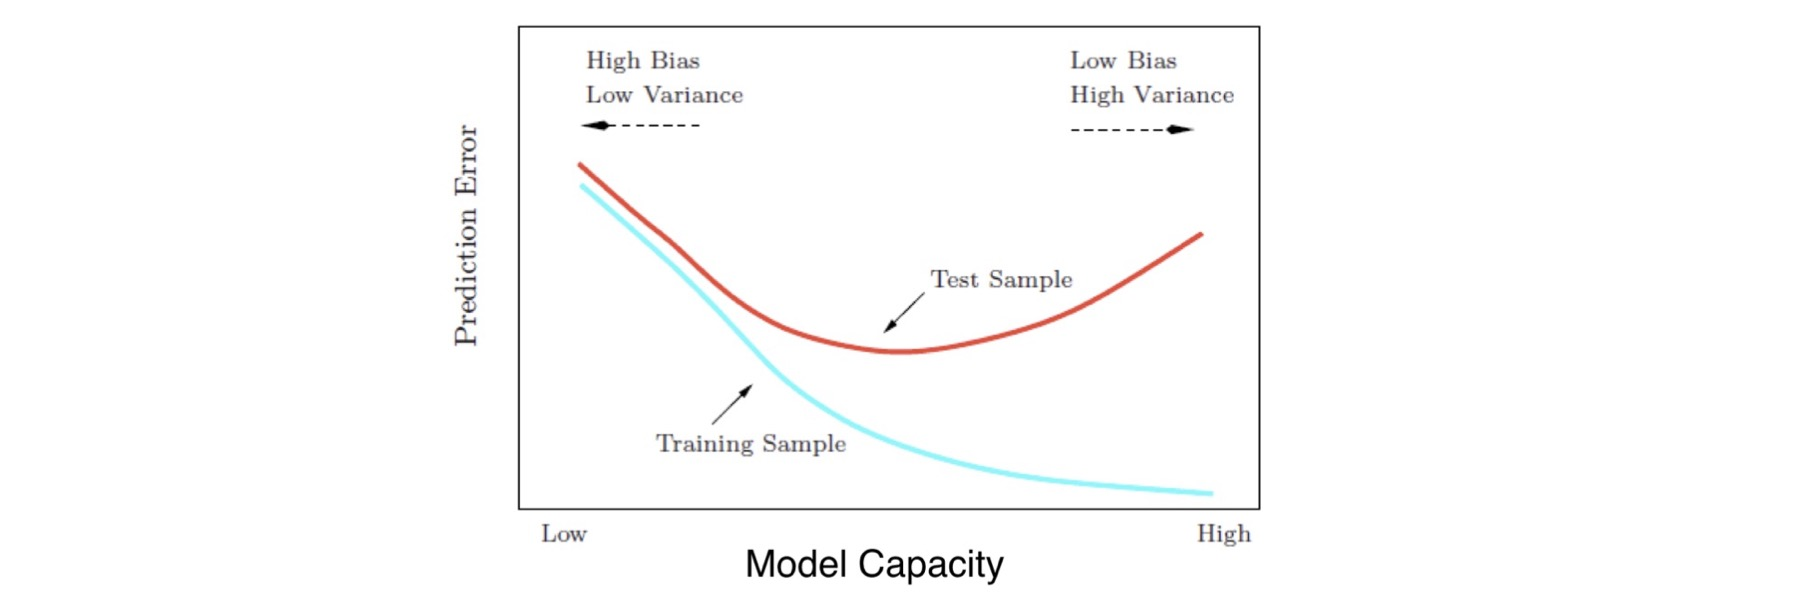
\includegraphics{../Figures/3. Overfitting.jpg}
\caption{Overfitting}
\end{figure}

    \hypertarget{note-2-workflow-for-optimizing-model-capacity}{%
\subsection{\texorpdfstring{\texttt{{[}note-2{]}} Workflow for
optimizing model
capacity}{{[}note-2{]} Workflow for optimizing model capacity}}\label{note-2-workflow-for-optimizing-model-capacity}}

\begin{itemize}
\item
  Start with a small network.
\item
  Gradually increase capacity.
\item
  Keep increasing capacity until the validation score is no longer
  improving.
\end{itemize}

    \hypertarget{note-3-sequential-experiments}{%
\subsection{\texorpdfstring{\texttt{{[}note-3{]}} Sequential
experiments}{{[}note-3{]} Sequential experiments}}\label{note-3-sequential-experiments}}

\begin{figure}
\centering
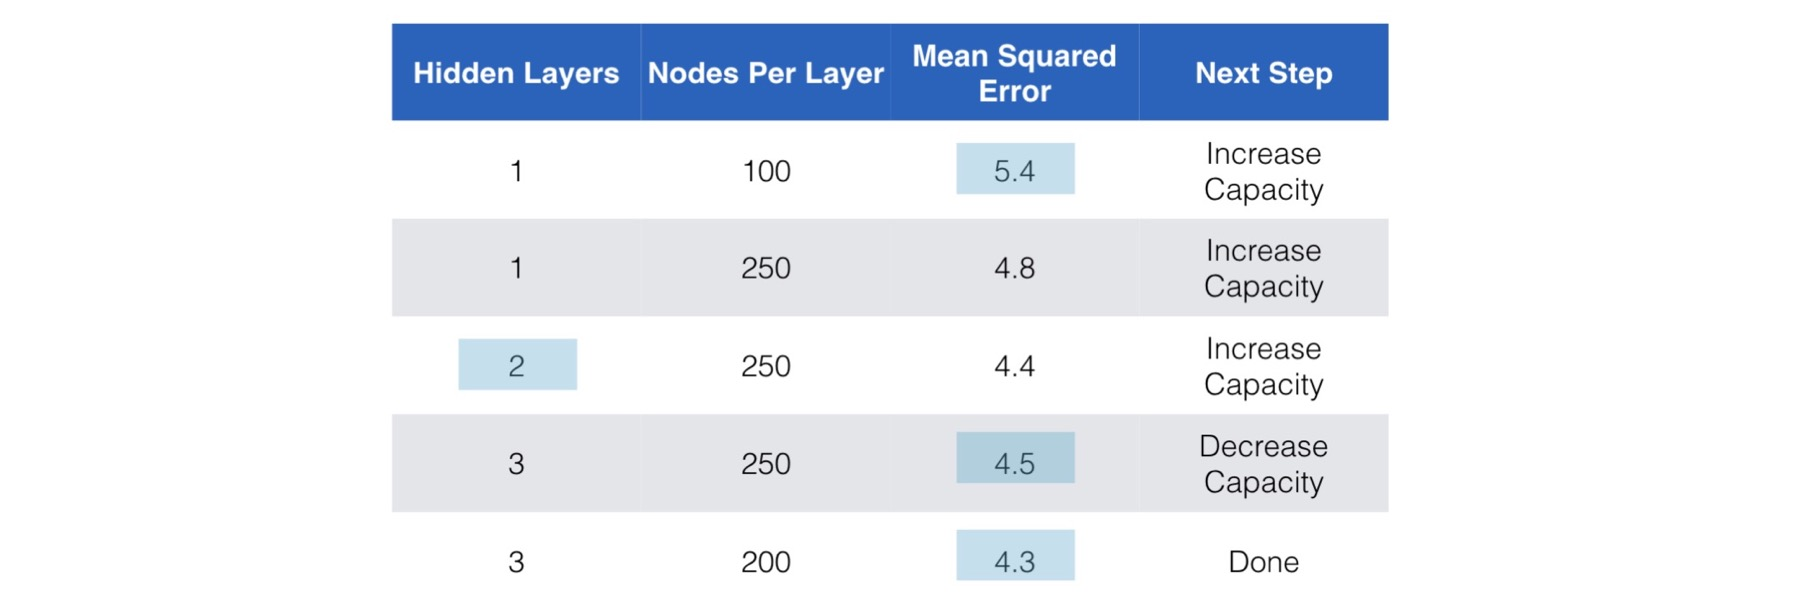
\includegraphics{../Figures/4. Sequential experiments.jpg}
\caption{Sequential experiments}
\end{figure}

    \hypertarget{quiz-1-experimenting-with-model-structures}{%
\subsection{\texorpdfstring{\texttt{{[}quiz-1{]}} Experimenting with
model
structures}{{[}quiz-1{]} Experimenting with model structures}}\label{quiz-1-experimenting-with-model-structures}}

\begin{itemize}
\item
  An experiment has run where has compared two networks that were
  identical except that the 2nd network had an extra hidden layer. It
  could be seen that this 2nd network (the deeper network) had better
  performance. Given that, which of the following would be a good
  experiment to run next for even better performance?

  \(\Box\) Try a new network with fewer layers than anything you have
  tried yet.

  \(\boxtimes\) Use more units in each hidden layer.

  \(\Box\) Use fewer units in each hidden layer.
\end{itemize}

    \hypertarget{stepping-up-to-images}{%
\section{Stepping up to images}\label{stepping-up-to-images}}

    \hypertarget{note-1-recognizing-handwritten-digits}{%
\subsection{\texorpdfstring{\texttt{{[}note-1{]}} Recognizing
handwritten
digits}{{[}note-1{]} Recognizing handwritten digits}}\label{note-1-recognizing-handwritten-digits}}

\begin{itemize}
\item
  MNIST dataset.
\item
  28 x 28 grid flattened to 784 values for each image.
\item
  Value in each part of the array denotes the darkness of that pixel.
\end{itemize}

\begin{figure}
\centering

\includegraphics{../Figures/5. Recognizing handwritten digits.jpg}
\caption{Recognizing handwritten digits}
\end{figure}

    \hypertarget{task-1-building-an-own-digit-recognition-model}{%
\subsection{\texorpdfstring{\texttt{{[}task-1{]}} Building an own digit
recognition
model}{{[}task-1{]} Building an own digit recognition model}}\label{task-1-building-an-own-digit-recognition-model}}

\(\blacktriangleright\) \textbf{Package pre-loading}

    \begin{tcolorbox}[breakable, size=fbox, boxrule=1pt, pad at break*=1mm,colback=cellbackground, colframe=cellborder]
\prompt{In}{incolor}{17}{\boxspacing}
\begin{Verbatim}[commandchars=\\\{\}]
\PY{k+kn}{import} \PY{n+nn}{pandas} \PY{k}{as} \PY{n+nn}{pd}
\PY{k+kn}{from} \PY{n+nn}{tensorflow}\PY{n+nn}{.}\PY{n+nn}{keras}\PY{n+nn}{.}\PY{n+nn}{layers} \PY{k+kn}{import} \PY{n}{Dense}
\PY{k+kn}{from} \PY{n+nn}{tensorflow}\PY{n+nn}{.}\PY{n+nn}{keras}\PY{n+nn}{.}\PY{n+nn}{models} \PY{k+kn}{import} \PY{n}{Sequential}
\PY{k+kn}{from} \PY{n+nn}{tensorflow}\PY{n+nn}{.}\PY{n+nn}{keras}\PY{n+nn}{.}\PY{n+nn}{utils} \PY{k+kn}{import} \PY{n}{to\PYZus{}categorical}
\end{Verbatim}
\end{tcolorbox}

    \(\blacktriangleright\) \textbf{Data pre-loading}

    \begin{tcolorbox}[breakable, size=fbox, boxrule=1pt, pad at break*=1mm,colback=cellbackground, colframe=cellborder]
\prompt{In}{incolor}{18}{\boxspacing}
\begin{Verbatim}[commandchars=\\\{\}]
\PY{n}{df} \PY{o}{=} \PY{n}{pd}\PY{o}{.}\PY{n}{read\PYZus{}csv}\PY{p}{(}\PY{l+s+s1}{\PYZsq{}}\PY{l+s+s1}{../Datasets/3. MNIST.csv}\PY{l+s+s1}{\PYZsq{}}\PY{p}{,} \PY{n}{header}\PY{o}{=}\PY{k+kc}{None}\PY{p}{)}
\PY{n}{X} \PY{o}{=} \PY{n}{df}\PY{o}{.}\PY{n}{iloc}\PY{p}{[}\PY{p}{:}\PY{p}{,} \PY{l+m+mi}{1}\PY{p}{:}\PY{p}{]}\PY{o}{.}\PY{n}{to\PYZus{}numpy}\PY{p}{(}\PY{p}{)}
\PY{n}{y} \PY{o}{=} \PY{n}{to\PYZus{}categorical}\PY{p}{(}\PY{n}{df}\PY{o}{.}\PY{n}{iloc}\PY{p}{[}\PY{p}{:}\PY{p}{,} \PY{l+m+mi}{0}\PY{p}{]}\PY{p}{)}
\end{Verbatim}
\end{tcolorbox}

    \(\blacktriangleright\) \textbf{Task practice}

    \begin{tcolorbox}[breakable, size=fbox, boxrule=1pt, pad at break*=1mm,colback=cellbackground, colframe=cellborder]
\prompt{In}{incolor}{19}{\boxspacing}
\begin{Verbatim}[commandchars=\\\{\}]
\PY{c+c1}{\PYZsh{} Create the model: model}
\PY{n}{model} \PY{o}{=} \PY{n}{Sequential}\PY{p}{(}\PY{p}{)}

\PY{c+c1}{\PYZsh{} Add the first hidden layer}
\PY{n}{model}\PY{o}{.}\PY{n}{add}\PY{p}{(}\PY{n}{Dense}\PY{p}{(}\PY{l+m+mi}{50}\PY{p}{,} \PY{n}{activation}\PY{o}{=}\PY{l+s+s1}{\PYZsq{}}\PY{l+s+s1}{relu}\PY{l+s+s1}{\PYZsq{}}\PY{p}{,} \PY{n}{input\PYZus{}shape}\PY{o}{=}\PY{p}{(}\PY{l+m+mi}{784}\PY{p}{,} \PY{p}{)}\PY{p}{)}\PY{p}{)}

\PY{c+c1}{\PYZsh{} Add the second hidden layer}
\PY{n}{model}\PY{o}{.}\PY{n}{add}\PY{p}{(}\PY{n}{Dense}\PY{p}{(}\PY{l+m+mi}{50}\PY{p}{,} \PY{n}{activation}\PY{o}{=}\PY{l+s+s1}{\PYZsq{}}\PY{l+s+s1}{relu}\PY{l+s+s1}{\PYZsq{}}\PY{p}{)}\PY{p}{)}

\PY{c+c1}{\PYZsh{} Add the output layer}
\PY{n}{model}\PY{o}{.}\PY{n}{add}\PY{p}{(}\PY{n}{Dense}\PY{p}{(}\PY{l+m+mi}{10}\PY{p}{,} \PY{n}{activation}\PY{o}{=}\PY{l+s+s1}{\PYZsq{}}\PY{l+s+s1}{softmax}\PY{l+s+s1}{\PYZsq{}}\PY{p}{)}\PY{p}{)}

\PY{c+c1}{\PYZsh{} Compile the model}
\PY{n}{model}\PY{o}{.}\PY{n}{compile}\PY{p}{(}\PY{n}{optimizer}\PY{o}{=}\PY{l+s+s1}{\PYZsq{}}\PY{l+s+s1}{adam}\PY{l+s+s1}{\PYZsq{}}\PY{p}{,}
              \PY{n}{loss}\PY{o}{=}\PY{l+s+s1}{\PYZsq{}}\PY{l+s+s1}{categorical\PYZus{}crossentropy}\PY{l+s+s1}{\PYZsq{}}\PY{p}{,}
              \PY{n}{metrics}\PY{o}{=}\PY{p}{[}\PY{l+s+s1}{\PYZsq{}}\PY{l+s+s1}{accuracy}\PY{l+s+s1}{\PYZsq{}}\PY{p}{]}\PY{p}{)}

\PY{c+c1}{\PYZsh{} Fit the model}
\PY{n}{model}\PY{o}{.}\PY{n}{fit}\PY{p}{(}\PY{n}{X}\PY{p}{,} \PY{n}{y}\PY{p}{,} \PY{n}{validation\PYZus{}split}\PY{o}{=}\PY{l+m+mf}{0.3}\PY{p}{)}
\end{Verbatim}
\end{tcolorbox}

    \begin{Verbatim}[commandchars=\\\{\}]
44/44 [==============================] - 1s 6ms/step - loss: 54.3641 - accuracy:
0.2529 - val\_loss: 7.2395 - val\_accuracy: 0.4925
    \end{Verbatim}

            \begin{tcolorbox}[breakable, size=fbox, boxrule=.5pt, pad at break*=1mm, opacityfill=0]
\prompt{Out}{outcolor}{19}{\boxspacing}
\begin{Verbatim}[commandchars=\\\{\}]
<tensorflow.python.keras.callbacks.History at 0x7f04e411e750>
\end{Verbatim}
\end{tcolorbox}
        
    \hypertarget{final-thoughts}{%
\section{Final thoughts}\label{final-thoughts}}

    \hypertarget{note-1-next-steps}{%
\subsection{\texorpdfstring{\texttt{{[}note-1{]}} Next
steps}{{[}note-1{]} Next steps}}\label{note-1-next-steps}}

\begin{itemize}
\item
  Start with standard prediction problems on tables of numbers.
\item
  Images (with convolutional neural networks) are common next steps.
\item
  \href{https://keras.io}{keras.io} for excellent documentation.
\item
  The graphical processing unit (GPU) provides dramatic speedups in
  model training times.
\item
  Need a CUDA-compatible GPU.
\end{itemize}

    \hypertarget{requirements}{%
\section{Requirements}\label{requirements}}

    \begin{tcolorbox}[breakable, size=fbox, boxrule=1pt, pad at break*=1mm,colback=cellbackground, colframe=cellborder]
\prompt{In}{incolor}{20}{\boxspacing}
\begin{Verbatim}[commandchars=\\\{\}]
\PY{k+kn}{from} \PY{n+nn}{platform} \PY{k+kn}{import} \PY{n}{python\PYZus{}version}
\PY{k+kn}{import} \PY{n+nn}{tensorflow} \PY{k}{as} \PY{n+nn}{tf}
\PY{k+kn}{import} \PY{n+nn}{matplotlib}

\PY{n}{python\PYZus{}version} \PY{o}{=} \PY{p}{(}\PY{l+s+s1}{\PYZsq{}}\PY{l+s+s1}{python==}\PY{l+s+si}{\PYZob{}\PYZcb{}}\PY{l+s+s1}{\PYZsq{}}\PY{o}{.}\PY{n}{format}\PY{p}{(}\PY{n}{python\PYZus{}version}\PY{p}{(}\PY{p}{)}\PY{p}{)}\PY{p}{)}
\PY{n}{pandas\PYZus{}version} \PY{o}{=} \PY{p}{(}\PY{l+s+s1}{\PYZsq{}}\PY{l+s+s1}{pandas==}\PY{l+s+si}{\PYZob{}\PYZcb{}}\PY{l+s+s1}{\PYZsq{}}\PY{o}{.}\PY{n}{format}\PY{p}{(}\PY{n}{pd}\PY{o}{.}\PY{n}{\PYZus{}\PYZus{}version\PYZus{}\PYZus{}}\PY{p}{)}\PY{p}{)}
\PY{n}{tensorflow\PYZus{}version} \PY{o}{=} \PY{p}{(}\PY{l+s+s1}{\PYZsq{}}\PY{l+s+s1}{tensorflow==}\PY{l+s+si}{\PYZob{}\PYZcb{}}\PY{l+s+s1}{\PYZsq{}}\PY{o}{.}\PY{n}{format}\PY{p}{(}\PY{n}{tf}\PY{o}{.}\PY{n}{\PYZus{}\PYZus{}version\PYZus{}\PYZus{}}\PY{p}{)}\PY{p}{)}
\PY{n}{matplotlib\PYZus{}version} \PY{o}{=} \PY{p}{(}\PY{l+s+s1}{\PYZsq{}}\PY{l+s+s1}{matplotlib==}\PY{l+s+si}{\PYZob{}\PYZcb{}}\PY{l+s+s1}{\PYZsq{}}\PY{o}{.}\PY{n}{format}\PY{p}{(}\PY{n}{matplotlib}\PY{o}{.}\PY{n}{\PYZus{}\PYZus{}version\PYZus{}\PYZus{}}\PY{p}{)}\PY{p}{)}

\PY{n}{writepath} \PY{o}{=} \PY{l+s+s1}{\PYZsq{}}\PY{l+s+s1}{../../requirements.txt}\PY{l+s+s1}{\PYZsq{}}
\PY{n}{requirements} \PY{o}{=} \PY{p}{[}\PY{p}{]}
\PY{n}{packages} \PY{o}{=} \PY{p}{[}\PY{n}{pandas\PYZus{}version}\PY{p}{,} \PY{n}{tensorflow\PYZus{}version}\PY{p}{,} \PY{n}{matplotlib\PYZus{}version}\PY{p}{]}

\PY{k}{try}\PY{p}{:}
    \PY{k}{with} \PY{n+nb}{open}\PY{p}{(}\PY{n}{writepath}\PY{p}{,} \PY{l+s+s1}{\PYZsq{}}\PY{l+s+s1}{r+}\PY{l+s+s1}{\PYZsq{}}\PY{p}{)} \PY{k}{as} \PY{n}{file}\PY{p}{:}
        \PY{k}{for} \PY{n}{line} \PY{o+ow}{in} \PY{n}{file}\PY{p}{:}
            \PY{n}{requirements}\PY{o}{.}\PY{n}{append}\PY{p}{(}\PY{n}{line}\PY{o}{.}\PY{n}{strip}\PY{p}{(}\PY{l+s+s1}{\PYZsq{}}\PY{l+s+se}{\PYZbs{}n}\PY{l+s+s1}{\PYZsq{}}\PY{p}{)}\PY{p}{)}
\PY{k}{except}\PY{p}{:}
    \PY{k}{with} \PY{n+nb}{open}\PY{p}{(}\PY{n}{writepath}\PY{p}{,} \PY{l+s+s1}{\PYZsq{}}\PY{l+s+s1}{w+}\PY{l+s+s1}{\PYZsq{}}\PY{p}{)} \PY{k}{as} \PY{n}{file}\PY{p}{:}
        \PY{k}{for} \PY{n}{line} \PY{o+ow}{in} \PY{n}{file}\PY{p}{:}
            \PY{n}{requirements}\PY{o}{.}\PY{n}{append}\PY{p}{(}\PY{n}{line}\PY{o}{.}\PY{n}{strip}\PY{p}{(}\PY{l+s+s1}{\PYZsq{}}\PY{l+s+se}{\PYZbs{}n}\PY{l+s+s1}{\PYZsq{}}\PY{p}{)}\PY{p}{)}

\PY{k}{with} \PY{n+nb}{open}\PY{p}{(}\PY{n}{writepath}\PY{p}{,} \PY{l+s+s1}{\PYZsq{}}\PY{l+s+s1}{a}\PY{l+s+s1}{\PYZsq{}}\PY{p}{)} \PY{k}{as} \PY{n}{file}\PY{p}{:}
    \PY{k}{for} \PY{n}{package} \PY{o+ow}{in} \PY{n}{packages}\PY{p}{:}
        \PY{k}{if} \PY{n}{package} \PY{o+ow}{not} \PY{o+ow}{in} \PY{n}{requirements}\PY{p}{:}
            \PY{n}{file}\PY{o}{.}\PY{n}{write}\PY{p}{(}\PY{n}{package} \PY{o}{+} \PY{l+s+s1}{\PYZsq{}}\PY{l+s+se}{\PYZbs{}n}\PY{l+s+s1}{\PYZsq{}}\PY{p}{)}

\PY{n}{max\PYZus{}characters} \PY{o}{=} \PY{n+nb}{len}\PY{p}{(}\PY{n}{python\PYZus{}version}\PY{p}{)}
\PY{k}{for} \PY{n}{package} \PY{o+ow}{in} \PY{n}{packages}\PY{p}{:}
    \PY{k}{if} \PY{n+nb}{max}\PY{p}{(}\PY{n}{max\PYZus{}characters}\PY{p}{,} \PY{n+nb}{len}\PY{p}{(}\PY{n}{package}\PY{p}{)}\PY{p}{)} \PY{o}{\PYZgt{}} \PY{n}{max\PYZus{}characters}\PY{p}{:}
        \PY{n}{max\PYZus{}characters} \PY{o}{=} \PY{n+nb}{max}\PY{p}{(}\PY{n}{max\PYZus{}characters}\PY{p}{,} \PY{n+nb}{len}\PY{p}{(}\PY{n}{package}\PY{p}{)}\PY{p}{)}

\PY{n+nb}{print}\PY{p}{(}\PY{l+s+s1}{\PYZsq{}}\PY{l+s+s1}{\PYZsh{}}\PY{l+s+s1}{\PYZsq{}} \PY{o}{*} \PY{p}{(}\PY{n}{max\PYZus{}characters} \PY{o}{+} \PY{l+m+mi}{8}\PY{p}{)}\PY{p}{)}
\PY{n+nb}{print}\PY{p}{(}\PY{l+s+s1}{\PYZsq{}}\PY{l+s+s1}{\PYZsh{}}\PY{l+s+s1}{\PYZsq{}} \PY{o}{*} \PY{l+m+mi}{2} \PY{o}{+} \PY{l+s+s1}{\PYZsq{}}\PY{l+s+s1}{ }\PY{l+s+s1}{\PYZsq{}} \PY{o}{*} \PY{p}{(}\PY{n}{max\PYZus{}characters} \PY{o}{+} \PY{l+m+mi}{4}\PY{p}{)} \PY{o}{+} \PY{l+s+s1}{\PYZsq{}}\PY{l+s+s1}{\PYZsh{}}\PY{l+s+s1}{\PYZsq{}} \PY{o}{*} \PY{l+m+mi}{2}\PY{p}{)}
\PY{n+nb}{print}\PY{p}{(}\PY{l+s+s1}{\PYZsq{}}\PY{l+s+s1}{\PYZsh{}}\PY{l+s+s1}{\PYZsq{}} \PY{o}{*} \PY{l+m+mi}{2} \PY{o}{+} \PY{l+s+s1}{\PYZsq{}}\PY{l+s+s1}{ }\PY{l+s+s1}{\PYZsq{}} \PY{o}{*} \PY{l+m+mi}{2} \PY{o}{+} \PY{n}{python\PYZus{}version} \PY{o}{+} \PY{l+s+s1}{\PYZsq{}}\PY{l+s+s1}{ }\PY{l+s+s1}{\PYZsq{}} \PY{o}{*}
      \PY{p}{(}\PY{n}{max\PYZus{}characters} \PY{o}{\PYZhy{}} \PY{n+nb}{len}\PY{p}{(}\PY{n}{python\PYZus{}version}\PY{p}{)} \PY{o}{+} \PY{l+m+mi}{2}\PY{p}{)} \PY{o}{+} \PY{l+s+s1}{\PYZsq{}}\PY{l+s+s1}{\PYZsh{}}\PY{l+s+s1}{\PYZsq{}} \PY{o}{*} \PY{l+m+mi}{2}\PY{p}{)}
\PY{k}{for} \PY{n}{package} \PY{o+ow}{in} \PY{n}{packages}\PY{p}{:}
    \PY{n+nb}{print}\PY{p}{(}\PY{l+s+s1}{\PYZsq{}}\PY{l+s+s1}{\PYZsh{}}\PY{l+s+s1}{\PYZsq{}} \PY{o}{*} \PY{l+m+mi}{2} \PY{o}{+} \PY{l+s+s1}{\PYZsq{}}\PY{l+s+s1}{ }\PY{l+s+s1}{\PYZsq{}} \PY{o}{*} \PY{l+m+mi}{2} \PY{o}{+} \PY{n}{package} \PY{o}{+} \PY{l+s+s1}{\PYZsq{}}\PY{l+s+s1}{ }\PY{l+s+s1}{\PYZsq{}} \PY{o}{*}
          \PY{p}{(}\PY{n}{max\PYZus{}characters} \PY{o}{\PYZhy{}} \PY{n+nb}{len}\PY{p}{(}\PY{n}{package}\PY{p}{)} \PY{o}{+} \PY{l+m+mi}{2}\PY{p}{)} \PY{o}{+} \PY{l+s+s1}{\PYZsq{}}\PY{l+s+s1}{\PYZsh{}}\PY{l+s+s1}{\PYZsq{}} \PY{o}{*} \PY{l+m+mi}{2}\PY{p}{)}
\PY{n+nb}{print}\PY{p}{(}\PY{l+s+s1}{\PYZsq{}}\PY{l+s+s1}{\PYZsh{}}\PY{l+s+s1}{\PYZsq{}} \PY{o}{*} \PY{l+m+mi}{2} \PY{o}{+} \PY{l+s+s1}{\PYZsq{}}\PY{l+s+s1}{ }\PY{l+s+s1}{\PYZsq{}} \PY{o}{*} \PY{p}{(}\PY{n}{max\PYZus{}characters} \PY{o}{+} \PY{l+m+mi}{4}\PY{p}{)} \PY{o}{+} \PY{l+s+s1}{\PYZsq{}}\PY{l+s+s1}{\PYZsh{}}\PY{l+s+s1}{\PYZsq{}} \PY{o}{*} \PY{l+m+mi}{2}\PY{p}{)}
\PY{n+nb}{print}\PY{p}{(}\PY{l+s+s1}{\PYZsq{}}\PY{l+s+s1}{\PYZsh{}}\PY{l+s+s1}{\PYZsq{}} \PY{o}{*} \PY{p}{(}\PY{n}{max\PYZus{}characters} \PY{o}{+} \PY{l+m+mi}{8}\PY{p}{)}\PY{p}{)}
\end{Verbatim}
\end{tcolorbox}

    \begin{Verbatim}[commandchars=\\\{\}]
\#\#\#\#\#\#\#\#\#\#\#\#\#\#\#\#\#\#\#\#\#\#\#\#\#
\#\#                     \#\#
\#\#  python==3.7.9      \#\#
\#\#  pandas==1.2.1      \#\#
\#\#  tensorflow==2.4.1  \#\#
\#\#  matplotlib==3.3.4  \#\#
\#\#                     \#\#
\#\#\#\#\#\#\#\#\#\#\#\#\#\#\#\#\#\#\#\#\#\#\#\#\#
    \end{Verbatim}


    % Add a bibliography block to the postdoc
    
    
    
\end{document}
